\def\mcirc{\mathbin{\scalerel*{\circ}{j}}}
\def\msquare{\mathord{\scalerel*{\Box}{gX}}}


\title{Реализация и применение строковых алгоритмов к задаче поиска
повторов в документации программного обеспечения}

\titlerunning{Применение ``полулокальных алгоритмов поиска``}

\author{Мишин Никита Матвеевич}

\authorrunning{Мишин Никита Матвеевич}

\tocauthor{Мишин Никита Матвеевич}
\institute{St Petersburg State University\\
	\email{mishinnikitam@gmail.com}}

\maketitle

\newcommand{\todo}[1]{{\color{red}{#1}}}
\newcommand{\new}[1]{{\color{blue}{#1}}}

\begin{abstract}
Данная работа посвящена исследованию применимости алгоритмов полулокального поиска наибольшей общей подпоследовательности и выравнивания строк (далее, просто ``полулокальные алгоритмы поиска``) для задач поиска повторов и групп повторов в документации программного обеспечения.
В работе представлен ряд алгоритмов поиска неточных повторов по заданному образцу на основе полулокальных алгоритмов поиска, в частности, разработана асимптотически более эффективная версия алгоритма из~\cite{luciv2019interactive}.
\end{abstract}

\section*{Введение}

% Абзац о том, что много документации ,она важна для разработки и сопровождения продуктов 
На сегодняшний день существует множество программных продуктов, и их количество с каждым годом лишь увеличивается.
% Вообще
Размер проектов исчисляется в строках кода и затраченных человеко-часах на соответствующую разработку.
Программные продукты часто могут содержать миллионы строк кода, на написание которых затрачены миллионы человеко-часов.
%\footnote{Код ядра линукса содержит более 27 млн строк кода, а на разработку ушло несколько сотен тысяч человеко-лет, 
%\emph{https://www.linux.com/news/linux-in-2020-27-8-million-lines-of-%code-in-the-kernel-1-3-million-in-systemd/, дата обращения 26.05.2020}}
%.
Соответственно, разработка и сопровождение таких сложных систем немыслимы без документации, количество которой лишь увеличивается.
% аналогичным образом растет с каждым новым продуктом.

% Детализируем, ссылками и мыслью, что качество документации важно и актуально
Важность сопроводительной документации не подвергается сомнению~\cite{kipyegen2013importance,chomal2014significance}.
Более конкретно, её качество напрямую влияет на жизненный цикл разработки системы, её конечную стоимость, время разработки, сопровождение, эксплуатацию и пр.~\cite{plosch2014value}. 
К критериям качества документации относятся точность, структурированность, последовательность изложения, понятность.
Иными словами, задачи поддержания качества документации (всех её критериев) на высоком уровне, а так же её написания, сопровождения и улучшения являются актуальными при создании, сопровождении и эксплуатации программных систем.
% Таким образом, различные виды программной документации играют важную роль в жизненном цикле разработки систем.

% Немного о клонах и их влиянии, -> их надо искать
Как в программном коде, так и в документации могут появляться \emph{текстовые повторы} (\emph{текстовые клоны}) или просто, \emph{повторы}.
\new{Текстовым повтором называется фрагмент текста, который присутствует в разных частях документа, возможно, с некоторыми незначительными изменениями.  Точным текстовым повтор называется текстовый повтор который присутствует в разных частях текста без изменений. Соответственно, неточный текстовый повтор --- с некоторыми изменениями. 

}
Влияние таких повторов на документацию различно.
% До сих пор нет четкого ответа на вопрос о влиянии \emph{текстовых повторов} на документацию.
К положительным факторам наличия повторов в документации можно отнести унификацию представления информации и создание общего контекста, что позволяет улучшить читаемость документации, её структурированность и передачу знаний (\emph{knowledge transfer}).
Несмотря на это, наличие повторов в документации влечет, как и в программном коде,  распространение ошибок и опечаток.
Процесс сопровождения документации усложняется при возникновении \emph{групп повторов}, т.е. множеств похожих фрагментов текста, при внесении изменения в один из которых, требуется внесение соответствующих изменений и в другие ``раскопированные'' элементы множества во избежание нарушения консистентности информации.
Более того, существующие исследования показывают~\cite{juergens2010can}, что повторы в документации программного обеспечения могут приводить и к появлению повторов в программном коде.
Таким образом, нахождение повторов в документации программного обеспечения является актуальной проблемой, а текущие исследования лишь подтверждают это утверждение~\cite{horie2010tool, poruban2014reusable, poruban2016preliminary, juergens2010can, oumaziz2017documentation}.

% Способы как ищут -> сводим к строковым алгоритмам
Важным этапом при решении задачи поиска повторов является выбор
% того, как будет измеряться похожесть двух текстовых фрагментов и что при выбранном подходе считать клонами.
меры, согласно которой будет измерятся \emph{схожесть} двух текстовых фрагметов, а так же критерия, согласно которому различные текстовые фрагменты будут считаться повторами.

% Существующие подходы можно разделить на несколько видов: лексикографическая похожесть, семантическая похожесть, синтаксически-лексическая похожесть и комбинация вышеперечисленных.
% К семантической похожести относятся подходы, при которых похожесть (или же расстояние между фрагментами) основывается на  их семантической близости, т.е на том, насколько одинаковый смысл несут эти фрагменты.
% Синтаксически-лексические подходы основываются на структурной и синтаксической похожести.
% При лексикографической похожести (с точностью до написания) учитывается лишь то, насколько посимвольно похожи два выбранных фрагмента.

Применение строковых алгоритмов является % наиболее
естественным подходом к поиску повторов как в произвольном тексте, так и в документации программного обеспечения.
Алгоритмы решения задач поиска наибольшей общей подпоследовательности~(\emph{LCS~--- longest common subsequence}) и выравнивания двух последовательностей~(\emph{SA~--- sequence alignment}) являются широко известными алгоритмами, которые имеют разные приложения, в том числе и к задаче поиска повторов.

LCS и SA измеряют то, насколько текстовые фрагменты похожи глобально (в общем) друг на друга. 
Интуитивно понятно, что этого бывает недостаточно, потому что часто два фрагмента бывают схожи лишь небольшой общей частью.
Решить эту проблему помогает обобщение на так называемый полулокальный случай, а именно, \emph{полулокальные задачи} поиска наибольшей общей подпоследовательности и выравнивания последовательностей (\emph{semi-local LCS, semi-local SA})~\cite{tiskin2006all}.
Автором данного обобщения является Тискин А.\,В., внёсший огромный вклад в развитие этой научной области~\cite{tiskin2015fast,tiskin2019bounded,krusche2009parallel,tiskin2006longest,tiskin2008semi,tiskin2011towards}.
В частности, им изобретены эффективные алгоритмы \new{для решения задач semi-local LCS и semi-local SA}.
Также на момент написания этой статьи, Тискин А.\,В заканчивал работу над фундоментальным трудом~\cite{tiskin2006all}, посвящённым теории полулокальных алгоритмов поиска и выравнивания последовательностей.


Тем не менее, несмотря на всю красоту и выдающиеся асимптотические свойства полулокальных алгоритмов, многие из них были описаны лишь теоретически и до конца не ясно, как именно они поведут себя на практике.
Недавние успехи в применении этих алгоритмов в области биоинформатики~\cite{baxter2012conserved,davies2015analysis, picot2010evolutionary} дают все основания полагать, что их можно успешно адаптировать и к задаче поиска повторов в документации программного обеспечения.
% Важно отметить, что большая часть алгоритмов ещё ни разу не была реализована на практике.

% В данной работе рассматривается адаптация
Данная работа посвящена адаптации алгоритмов решения полулокальных задач поиска наибольшей общей подпоследовательности и выравнивая строк к задаче поиска повторов в документации программного обеспечения.
%В данной работе представлено решение задачи поиска повторов в документации с помощью применения и адаптации алгоритмов решения задач \emph{semi-local lcs} и \emph{semi-local sa}.
Адаптированные алгоритмы разработаны и реализованы в виде библиотеки на языке \textsc{Kotlin}.
% Для оценки применимости решения была осуществлена реализация приложения и библиотеки алгоритмов.
Апробация результатов произведена на {API}-документации.


\section{Обзор}
\label{sec:overview}
В этой главе представлен обзор предметной области, в частности работ, связанных с повторами в документации программного обеспечения (ПО), описана модель повторов, которая будет использована в дальнейшем. 
Исходя из текущих исследований, сформулированы задачи поиска повторов в документации ПО.
Также произведено исследование полулокальных задач поиска наибольшей общей подпоследовательности и выравнивания строк, описаны решающие их алгоритмы, % и идеи со свойствами, лежащими за ними.
идеи, лежащие в их основе, а также присущие им свойства.

\subsection{Повторы в документации ПО}\label{duplicateReport}

За последние десять лет появилось множество работ, посвященных разработке, усоверщенствованию и поддержке документации ПО, в частности проблемам, связанным с наличием и выявлением в ней повторов.
Одни работы посвящены эмпирическим исследованиям о количестве повторов  в различных видах документации ПО~\cite{poruban2016preliminary,juergens2010can,oumaziz2017documentation}, другие~---~фокусируются на реализации механизма переиспользования повторяющихся фрагментов информации в документации~\cite{koznov2015clone,horie2010tool,poruban2014reusable}, третьи~---~на алгоритмах и подходах поиска повторов~\cite{luciv2018detecting,luciv2019interactive,blasi2018replicomment,rago2016identifying, soto2015similarity}.

Юргенсен Э. и др.~\cite{juergens2010can} провели широкомасштабное исследование спецификаций требований различных проектов \new{на предмет наличия повторов}. 
Их исследование показало, что количество повторов может быть значительно (вплоть до 70\%). 
Стоит отметить, что они адаптировали \textsc{CONQAT}\footnote{\url{https://www.cqse.eu/}}~---~инструмент, предназначенный для непрерывной оценки качества документации, ---~ к задаче поиска повторов.
В их неформальной модели, повтор~---~это часть (подстрока) спецификации, которая повторяется более двух раз, а в группу объединяются те повторы, которые разделяют общую часть.
Стоит отметить, их адаптированное решение находит исключительно точные\todo{а было где-то написано про точные и неточные?}\new{в начале теперь упомянул} повторы.

Носаль М. и др.~\cite{poruban2016preliminary} провели эмпирическое исследование пяти крупных \textsc{JavaDoc} проектов, целью которого являлось проверка гипотезы о том, что комментарии к коду содержат большое количество повторов.
Саму модель повторов они определили неформально, а инструмент для нахождения повторов\footnote{\textsc{CPD} (copy-paste detector) инструмент на основе строкового алгоритма Рабина--Карпа, который позволяет находить только точные повторы.} адаптировали.
Результаты их работы подтвердили гипотезу исследования. 

Работа Умазиза М.\, А. и др.~\cite{oumaziz2017documentation} также относится к эмпирическому исследованию \textsc{JavaDoc} проектов. 
Их работа мотивирована критической важностью документации программного кода в процессе разработки ПО.
В работе повторы рассматриваются как цельные \textsc{JavaDoc} комментарии, которые встречаются в документации более одного раза, иными словами, рассматривается неформальная модель точных повторов.
Для нахождения повторов был адаптирован инструмент \textsc{GumTree} tool\footnote{\url{https://github.com/GumTreeDiff/gumtree}}, предназначенный для анализа программного кода на основе построения синтаксических деревьев.
Результаты исследования показали, что разработчики часто переиспользуют части документации.
Также их исследование показало, что текущие инструменты для работы с \textsc{JavaDoc} документацией не позволяют в полной мере избавиться от повторов.

%запашок
% В работе~\cite{blasi2018replicomment} авторами создан прототип инструмента \emph{RepliComment} для нахождения точных повторов в \emph{JavaDoc} документации, точнее комментариях к методам (использована неформальная модель повторов).
% Также инструмент позволяет классифицировать найденные решения, что позволило исследователям найти ряд ошибок и неточностей и, как следствие, улучшить качество документации (они отправили разработчикам список найденных ошибок и неточностей).
% В итоге,  результаты анализа нескольких проектов c помощью \emph{RepliComment} показали, что как код может иметь ``плохой запах'' (code smelss), так и комментарии к нему. 
% и его достаточно много т.е в комментариях может содержаться много повторов.

% Авторы~\cite{rago2016identifying} так же, как и~\cite{juergens2010can}, делают акцент работы на повторах в спецификации требований, в частности на повторах функциональных требований в \emph{use-case} диаграммах.
% Для анализа этого вида документации они реализовали комплексный инструмент  \emph{RegAligner}, который использует комбинированный подход для детектирования повторов.
% Подход основан на конвейерной архитектуре. 
% На первом этапе применяются техники обработки естественного языка (nlp), затем используется метод машинного обучения для трансляции результатов в промежуточный язык. Таким образом, получается множество цепочек, которые попарно выравниваются.
% \emph{ReqAligner} в силу своего подхода позволяет находить не только точные повторы, но и семантически схожие.
% Также необходимо отметить, что авторы не определили формальной модели повторов.
% Авторы провели апробацию инструмента на нескольких спецификациях, получив в результате 86\% полноту и 63\% точность.
% Их результаты апробации также подтвердили факт наличия повторов в \emph{use-case} диаграммах.


Луцив Д.\,В. и коллеги внесли большой вклад своими исследованиями в области поиска повторов в документации ПО~\cite{luciv2018detecting,luciv2018duplicate,luciv2019interactive,koznov2015clone,koznov2017duplicate,luciv2016fuzzy}. 
Они разработали комплексный инструмент \textsc{Duplicate Finder}, позволяющий находить повторы в документации, визуализировать их, а так же вносить изменения в исходную документацию.
Более того, они разработали формальную модель повторов в документации ПО и на ее основе создали алгоритмы для поиска как повторов по заданному шаблону, так и для выявления групп повторов.
Формальная модель позволила им доказать ряд свойств в отношении этих алгоритмов.

Алгоритм поиска групп повторов~\cite{luciv2016fuzzy} основан на \todo{надо бы пояснить, так ниже в абазцае идея описана - Сперва находятся все точные повторы ....} идее искусственного конструирования повторов.
Сперва находятся все точные повторы, а затем на их основе строятся группы неточных повторов.
Такая интерпретация происхождения неточных повторов имеет право на жизнь, но она искусственна, что справедливо приводит к высокому уровню \new{ложно-положительных срабатываний при нахождении повторов в их результатах апробации.}
% Про цельность?

% Несмотря на то, что представленный алгоритм обладает приемлемыми характеристиками, он игнорирует семантику выделяемых повторов, что оказывается
% важным для практических применений

Алгоритм поиска повторов по образцу~\cite{luciv2019interactive} основан на идее так называемого \emph{скользящего окна}.
Сперва находятся все похожие фрагменты, а затем производится их фильтрация и сжатие.
Асимптотика алгоритма оценивается как $max(O(|t|\times|p|^4),\ O(|t|\times \log |t|))$, где $t$~---~текст, а $p$~---~шаблон.
Авторами доказана полнота алгоритма.
Несмотря на это, такая асимптотическая оценка делает его не применимым на потенциально больших данных.
\new{
Также алгоритм обладает полнотой лишь при условии использования редакционного расстояния, что  ограничивает применение других метрик и схем подсчета похожести между двумя текстовыми фрагментами.} 

Таким образом, во-первых, для различных видов документации, в частности \textsc{JavaDoc} документации, задача поиска повторов является как никогда актуальной.
Во-вторых, несмотря на большое количество работ, посвященных  данной тематике, существующие подходы и алгоритмы могут быть улучшены как в теоретических оценках, так и на практике.
В-третьих, в работах преобладает неформальная модель повторов.
Наконец, исследователи помимо нахождения пар повторов, также ищут как группы повторов, так и осуществляют поиск повторов по образцу.


\subsection{Модель повторов в документации ПО}\label{Model}
% добавить про модели
Как было описано выше, существует множество неформальных моделей, по-разному определяющих понятие повтора в документации ПО.
% что такое \emph{повторы}.
% Можно сказать более точно, в каждой статье дается свое (авторское) видение.
Более того, в каждой статье даётся своё, авторское, видение.
Формальная \todo{плохое слово модель здесь, каджется,}\new{не придумал лучше, а почему нет?} модель присутствует только в работах Луцива Д.\,В. и соавторов.
% моделей меньше, если не сказать немного.

В данной работе будет использована наиболее общая модель, согласно которой повтор~--- это отношение между двумя непересекающимися фрагментами $a$ и $b$, которое задается с помощью функции \todo{похожести} $g$, \new{ которая измеряет меру подобия двух фрагментов}.
Отметим, что в данной модели не накладывается никаких ограничений на саму функцию $g$.
Например, в качестве $g$ можно выбрать функцию, которая высчитывает количество одинаковых символов в двух фрагментах и сравнивает его с некоторым предопределённым пороговым значением. %$h$.
Заметим, что в этом случае функция симметрична по отношению к своим аргументам, т.е. $g(a,b) = g(b,a)$.
% Например, из того, что  фрагмент $a$ является повтором фрагмента $b$, может не следовать то, что $b$ также является повтором $a$ (функция может быть не симметрична по отношению к своим аргументам, т.е $g(a,b) \neq  g(b,a)$). 

% a->b b->c   d->c  -> a,b,c,d
% GOVNO PRAV

Набор повторов может образовывать \emph{группу повторов}, если он удовлетворяет определенным свойствам. Иными словами, группа повторов~---~это множество повторов, которые в совокупности удовлетворяют заданному предикату.
Предикатом может служить следующее утверждение: ``В графе, построенном по группе повторов, существует хотя бы одна вершина, из которой достижимы все остальные. Вершинами графа являются повторы, рёбра~---~значение функции $g$ для выбранных вершин.''
% TODO/Заметим, что модель (или не может?) является частным случаем (удалить?) .


\subsection{Задачи поиска повторов в документации ПО}

Можно выделить несколько задач относящихся к поиску повторов в документации ПО:
\begin{itemize}
\item поиск всех повторов,
\item поиск групп повторов,
\item поиск повторов по образцу.
\end{itemize}

\paragraph{Поиск всех повторов}
Задача поиска всех пар повторов формулируется следующим образом: в данном наборе текстов $t$ необходимо найти все пары повторов, согласно выбранной функции $g$.

\paragraph{Поиск групп повторов}
Задача поиска групп повторов формулируется следующим образом:
В данном наборе текстов $t$ необходимо найти все непересекающиеся группы повторов согласно выбранной функции $g$ и предикату $\gamma$.
Эта задача является вариацией предыдущей задачи.

\paragraph{Поиск по образцу}
Задача поиска по образцу формулируется следующим образом:
пусть даны шаблон $p$ и набор текстов $t$, необходимо найти все непересекающиеся повторы шаблона $p$ в тексте $t$ согласно выбранной функции  $g$.
\new{Удалить мб просто}
\todo{кривая фраза: }Стоит отметить, что могут существовать разные способы \todo{разбиения на непересекающиеся повторы}.

% Над набором javaDoc комментариев нужно построить группы повторов, иными словами найти такое разбиение
% Задачу поиска групп повторов в Javadoc документации
% The semi-local LCS problem represents a generalization of a well-knownLCS problem. It is defined as follows

% В данном разделе представлены базовые математические модели и
% определения, использующиеся при решении поставленной задачи, даны
% определения метрик качества стабилизации видео, которые задействованы в алгоритмах стабилизации и калибровки, а также описан метод
% сбора тестовых данных и их форма
% \subsection{Документация ПО}

% \subsubsection{Виды документации ПО}
% % табличка должна быть


\subsection{Полулокальные задачи поиска}

В этой секции приведены общие сведения о полулокальных задачах поиска наибольшей общей подпоследовательности и выравнивания строк.
Полное описание задач, теорем, а также доказательств их свойств, может быть найдено в~\cite{alex2007semilocal}.

% рассказать про lcs и sa
\subsubsection{Задачи поиска наибольшей общей подпоследовательности (LCS) и выравнивания строк (SA)}\mbox{}

Для начала, необходимо дать определение, что такое \emph{LCS} и \emph{SA}.

\begin{definition}[Задача о наибольшей общей подпоследовательности (LCS)]
Даны две строки $a$ и $b$ длин $m$ и $n$ соответственно.
Необходимо найти наибольшую общую подпоследовательность символов для строк $a$ и $b$, а именно значение длины этой подпоследовательности, т.е. $LCS$-значение.
\end{definition}
% \paragraph*{Задача о наибольшей общей подпоследовательности (LCS)}\mbox{}
%% Даны две строки $a$ и $b$ длин $m$ и $n$ соответственно.
%% Необходимо найти наибольшую общую подпоследовательность
%% %\footnote{Тоже, что и в математике.
%% %Подпоследовательность~--- это последовательность, которая может быть получена из другой последовательности путем удаления части ($\geq 0$) её элементов без изменения порядка следования элементов.}
%%  символов для строк $a$ и $b$, а именно значение длины этой подпоследовательности т.е $lcs$-значение.
%% Пример:

Пример: \hspace{1cm}
%\begin{center}
    $LCS(abbba,aa)=aa$ (её длина 2).
%\end{center}
 
%\paragraph*
% \subsubsection{Задача о выравнивании двух последовательностей (SA)}\mbox{}
\begin{definition}[Задача о выравнивании двух последовательностей (SA)]
Даны две строки $a$ и $b$ длин $m$ и $n$ соответственно.
Необходимо найти наибольшее  значение функции выравнивания двух строк ($SA$) с учетом выбранной схемы оценки $w = (w_{+}, w_{0} ,$ $w_{-})=$ (пара символов совпала, пара символов не совпала, символ выровнен по пропуску).
Схема оценки отвечает за учет стоимости выравнивания пары символов из соответствующих строк, а сама функция выравнивания определяется следующим образом:
\begin{equation}\label{formula:sa}
\begin{array}{ll}
  SA(a,b,w) &= w_{+}k^{+} + w_{0}k^{0} + w_{-} (m + n - 2k^{+} - 2k^{0}) \\
  &= k^{+} (w_{+} - 2w_{-} ) + k^{0}  (w_{0} - 2w_{-}) + w_{-}(m + n),
\end{array}
%\end{aligned}
\end{equation}
где $k^{+}$ и $k^{0}$~--- количество совпадающих и несовпадающих пар символов в выравнивании.
\end{definition}

Иными словами, когда две строки выровнены, пара соответствующих символов $\gamma$ из $a$ и $\beta$ из $b$ будет называться \emph{выровненной}.
Символы в паре могут совпасть ($w_{+}$), а могут быть различны ($w_{0}$).
Также при выравнивании символ одной строки может  быть выровнен не по символу из другой строки, а по так называемому пропуску ($gap$, $w_{-}$), т.е. при выравнивании происходит разрыв и ставится пропуск '-'.
Пример выравнивания для строк $a=ABCA$, $b=ACBA$ и схемы оценки $w = (1, -0.3, -0.5)$:
\begin{center}
    \begin{tabular}{ccccc}
    A & - & B &  C  &  A \\
    A & C & B &  - &  A
    \end{tabular}
\end{center}
Здесь результат выравнивания $SA(a,b) = 3*1.0-2*0.5 = 2.0$.

Заметим, что задача поиска наибольшей подпоследовательности является частным случаем задачи выравнивания строк при схеме подсчёта $(1,0,0)$.
Обе описанные задачи решаются с помощью динамического программирования и имеют асимптотическую сложность $O(m \times n)$~\cite{huang1994global}.
% Заметим, что обе задачи сводятся к поиску на прямоугольной решетке (графе) пути между  наибольшего значения  ${\color{red} Вставить картинку   }$.

Как было отмечено во введении, решения задач LCS и SA позволяют найти насколько в глобальном смысле похожи заданные строки.
Во многих задачах интересны так называемые локальные и полулокальные случаи.
Локальный случай относится к нахождению таких пар участков из строк $a$ и $b$, которые максимально похожи друг на друга.
Описание полулокальных задач приведено ниже.
% Полулокальный же вариант --- это, то , что лежит между глобальным и полностью локальным случаем.
% \begin{algorithm}
% \caption{Префикс SA (LCS)}\label{alg:lcssa}
% Вход: строки $a$ и $b$ длин $m$ и $n$ соответственно\\
% Выход: наибольшее значение функции \emph{sa} (\emph{lcs}) для всех пар префиксов, в частности для $a[0:n]$ и $b[0:n]$\\
% Комментарии: матрица $h$ хранит соответствующие значения т.е элемент матрицы $h[i,j]$ хранит наибольшее значение \emph{sa} (\emph{lcs}) для префиксов строк $a[0:i]$ и  $b[0:j]$\\
% Псевдокод: 
% \begin{algorithmic}[1]
% \State $h[0, j] := 0$ для всех $j \in 0..n$ 
% \State $h[i, 0] := 0$ для всех $i \in 0..m$
% \For{i in 0...m}
% \For{j in 0 ..n}
% \State $h[i,j] := max \begin{cases}
% 			h[i-1,j-1] +  
% 			\begin{cases}
% 			w_{+}, & \text{если $a[i]= b[j]$} \\
% 			w_{0}, &  \text{если $a[i]\neq b[j]$}
% 			\end{cases}, & \text{} \\
%             h[i-1,j] + w_{-}, & \text{} \\
%             h[i,j-1] + w_{-}, & \text{}
% 		 \end{cases}$
% \EndFor
% \EndFor
% \end{algorithmic}
% \end{algorithm}


% \subsubsection{Semi-local LCS и SA}

% Semi-local LCS def
\begin{definition}[Задача поиска полулокальной наибольшей общей подпоследовательности (semi-local LCS)]
Пусть даны две строки $a$ и $b$ длин $m$ и $n$ соответственно. 
Необходимо найти значение $LCS$ для следующих подзадач:
\begin{itemize}
\item \textbf{string-subtring}: для каждой из подстрок строки $b$ найти наибольшую общую подпоследовательность со строкой $a$, а именно значение $LCS$;
\item \textbf{subtring-string}: для каждой из подстрок строки $a$ найти наибольшую общую подпоследовательность со строкой $b$, а именно значение $LCS$;
\item \textbf{prefix-suffix}: для каждой пары, состоящей из префикса строки $a$ и суффикса строки $b$, найти наибольшую общую подпоследовательность;
\item \textbf{suffix-prefix}: для каждой пары, состоящей из префикса строки $b$ и суффикса строки $a$, найти наибольшую общую подпоследовательность.
\end{itemize}
\end{definition}

Решение данной задачи представляется в виде квадратной матрицы $H_{a,b}$, где каждый квадрант отвечает за одну из описанных подзадач: 
\begin{equation}
H_{a,b} = \begin{bmatrix}
  suffix-prefix & substring-string \\
  string-substring & prefix-suffix
  \end{bmatrix}.
\end{equation}

Более того, каждая ячейка содержит ответ для заданной пары подстрок.
Таким образом, сразу очевиден наивный алгоритм решения задачи~---~последовательное заполнении ячеек матрицы, асимптотическая сложность которого $O((n+m)^2) \times O((n+m)^2) = O((n+ m)^4)$.

К счастью, разработанная теория вокруг данной задачи позволяет её решать намного эффективнее.
% Точнее,
Существует несколько алгоритмов, имеющих асимптотическую сложность $O(n \times m)$ и $O(n \times m \times \log n)$ соответственно.
Данные алгоритмы опираются на свойства матрицы $H_{a,b}$. %, которыми она обладает.
% Все они основаны на свойствах матрицы $H_{a,b}$ и теоремах связанных  с ней.
Во-первых, по построению, матрица относится к классу так называемых юнит aнти-матриц Монжа.
\begin{definition}[(Aнти-)матрицей Монжа (unit anti-Monge)]
Матрица $H$ называется (анти-)матрицей Монжа, если %выполняется следующее:
\begin{equation}
  H[i, j] + H[i^{'},j^{'}] \leq(\geq) H[i', j] + H[i,j'] ,\quad \forall \: i \leq i' , j \leq j'.
\end{equation}
\end{definition}

\begin{definition}[Юнит (анти)-матрицей Монжа](Анти-)матрица Монжа $H$ называется \emph{юнит (анти)-матрицей Монжа}, если матрица (-)$H^{\msquare}$, получающаяся в результате взятия перекрёстной разности анти-диагонали и диагонали для всех смежных квадратов 2 на 2, является перестановочной.
\end{definition}
Например, следующая (первая) матрица является юнит матрицей Монжа:
\begin{equation}
\begin{bmatrix}
0 & 2 & 3 \\
0 & 1 & 2 \\
0 & 1 & 1
\end{bmatrix} ^ { \msquare} =
\begin{bmatrix}
(2 + 0) - (1 + 0)  & (3 + 1) - (2 + 2)  \\
(1 + 0) - (1 + 0) &  (2 + 1) - (1 + 1) 
\end{bmatrix} = 
\begin{bmatrix}
1 & 0  \\
0 & 1 
\end{bmatrix} 
\end{equation}

Во-вторых, данный класс матриц образует моноид с операцией $\otimes$ над этими матрицами, которая известна как \emph{distance matrix multipliсation}\footnote{Операция над матрицами в тропической алгебре. Это обычное матричное умножение, в котором умножение $(*)$ заменено на сложение $(+)$, а сложение $(+)$~---~на операцию взятия минимума $(min)$.}.

В-третьих, доказано~\cite{tiskin2006all}, что можно произвести декомпозицию данной матрицы и хранить её неявно в виде перестановочных матриц $P_{a,b}$, так называемое \emph{ядро} матрицы $H_{a,b}$, что позволяет существенно сократить объем используемой памяти.
Эти ядра также образуют моноид, называемый \emph{моноидом липких кос}, для которых также определена своя операция умножения $\odot$.
Удивительным образом, эти два моноида изоморфны друг другу~\cite{tiskin2006all}, что позволяет использовать $\odot$ вместо $\otimes$. 
Иными словами, для того, чтобы посчитать произведение двух матриц Монжа, можно перейти к косам, произвести над ними операцию $\odot$, тем самым получив результат исходной задачи; справедливо и обратное для липких кос и операции $\otimes$.
    
% В-четвертых, доказано~\cite{tiskin2006all}, что
Наконец, ядро $P_{a,b}$ может быть выражено через конкатенацию двух меньших решений~\cite{tiskin2006all}:
\begin{equation}\label{formulaKernelCompistion}
P_{a,b}  = P_{a^{'},b} \odot P_{a^{''},b}, a  := a^{'}a^{''}.
\end{equation}
Это позволяет использовать известный принцип ``\emph{разделяй и властвуй}''.

Стоит отметить, что Тискиным А.\,B. изобретен быстрый алгоритм для перемножения двух липких кос~---~\emph{алгоритм муравья}~\cite{tiskin2015fast}, имеющий асимптотическую сложность $O(n \times \log n)$, где $n$~---~количество ненулевых элементов в перестановочной матрице.
Тем не менее, 
% Однако
неясно, насколько практическая реализация данного алгоритма будет эффективна на практике.

Из всего вышесказанного сразу вытекают следующие два рекурсивных алгоритма, основанные на умножении липких кос и
% монжевого матричного умножения
умножения матриц Монжа через $\otimes$~\cite{tiskin2008semi}.
% algo implitic
 \begin{algorithm}[h]
 \caption{Рекурсивный алгоритм для решения semi-local lcs через липкое умножение кос}\label{alg:ant}
 Вход: строки $a$ и $b$ длин $m$ и $n$ соответственно\\
 Выход: ядро  матрицы $H_{a,b}$\\
 Комментарии: Сложность алгоритма $O(n \times m)$\\
 Псевдокод:

% % , не имеет практической реализации
 \begin{algorithmic}[1]
 \If {$n=1$ и $m=1$}    \Comment{База рекурсии, длина строк 1}
     \If{$a=b$}
         \State Вернуть ядро  $2 \times 2$, отвечающее диагональной
         \par\hskip\algorithmicindent
         единичной матрице
     \Else
         \State Вернуть ядро размера 2 на 2, отвечающее  
         \par\hskip\algorithmicindent антидиагональной единичной матрице
     \EndIf
 \Else
     \State Выбрать строку с наибольшей длиной
     \State Разбить её на конкатенацию двух подстрок
     \State Рекурсивно запустить алгоритм над этими двумя половинами
     \State Произвести конкатенацию решений через  $\odot$     
     \State Вернуть полученное решение
 \EndIf
 \end{algorithmic}
% % Стоит отметить, что неизвестно, насколько данный алгоритм эффективен на практике, поскольку он не не имеет практической реализации.
 \end{algorithm}
% algos explciit
 \begin{algorithm}[h]
 \caption{Рекурсивный алгоритм для решения semi-local lcs через явное умножение матриц}\label{alg:monge}
 Вход: строки $a$ и $b$ длин $m$ и $n$ соответственно\\
 Выход:  матрица $H_{a,b}$\\
 Комментарии: Сложность алгоритма $O(n \times m \times \log n)$\\
 Псевдокод:

 \begin{algorithmic}[1]
 \If {$n=1$ и $m=1$}    \Comment{База рекурсии, длина строк 1}
     \If{$a=b$}
         \State Вернуть матрицу, которой отвечает ядро размера 2 на 2,
         \par\hskip\algorithmicindent единичная диагональная матрица
     \Else
         \State Вернуть матрицу, которой отвечает ядро размера 2 на 2,
         \par\hskip\algorithmicindent единичная анти-диагональная матрица
     \EndIf
 \Else
     \State Выбрать строку с наибольшей длиной
     \State Разбить её на конкатенацию двух подстрок
     \State Рекурсивно запустить алгоритм над этими двумя половинами
     \State Произвести конкатенацию найденный решений через  $\otimes$ 
     % (умножение через алгоритм swamk )
     \State Вернуть полученное решение
 \EndIf
 \end{algorithmic}
 \end{algorithm}

% В силу того, что матрица $H$--- уни анти монжева, и выполняется (5), и благодаря изоморфизму можно восопльзоваться быстрым умножением монжевых матриц котороые основано на smawk алгоритме.
% Это позволяет добиться сложности $O(n \times m)$.

Также существует итеративный алгоритм, имеющий асимптотическую сложность $O(n \times m)$, основанный на распутывании кос\footnote{С каждой перестановочной матрицей размера $n \times n$ ассоциирована \emph{сокращенная липкая коса} (\emph{reduced sticky braid}). Одной сокращенной липкой косе соответствует бесконечное множество липких кос. Таким образом, произвольную липкую косу можно \emph{распутать} до (свести к) сокращенной, которой уже будет отвечать ядро $P_{a,b}$.
}.

% Факт того, что ядро $P_{a,b}$ относится к \emph{моноиду липких кос}, позволяет решить задачу \emph{semi-local lcs} неявно через операцию распутывания кос, которая 
% через так называемое сведение косы к 
% Также, из-за того, что 
% существует итеративный алгоритм, основанный на том факте, что \emph{липкую косу}, можно встроить в  
% Также стоит упомянуть, известный еще с годов итеративный алгоритм~\cite{alavaes}, который также позволяет решить задачу за $O(n \times m)$  

% Еще раз отметим, что
Для простоты изложения некоторые детали при описании могут быть опущены.
Подробное описание можно найти в~\cite{alex2007semilocal}.

% Таким образом, часть из упомянутых  алгоритмов позволяют решать за ту же асимптотику что и обычный \emph{lcs}.
%  рассказать про semi local
% Аналогичным образом присутствует обобщение на полулокальную версию выравнивания строк  (semi-local sa).
% Semi-local SA def

\begin{definition}[Задача поиска полулокального выравнивания двух строк (semi-local SA)]
Даны две строки $a$ и $b$ длин $m$ и $n$ соответственно, а также схема оценки $w = (w_{+}, w_{0} , w_{-})$. 
Необходимо найти значение выравнивания ($SA$) для следующих подзадач:
\begin{itemize}
\item \textbf{string-subtring}: для каждой из подстрок строки $b$ найти максимальное выравнивание со строкой $a$;
\item \textbf{subtring-string}: для каждой из подстрок строки $a$ найти максимальное выравнивание со строкой $b$;
\item \textbf{prefix-suffix}: для каждой пары, состоящей из префикса строки $a$ и суффикса строки $b$, найти максимальное выравнивание;
\item \textbf{suffix-prefix}: для каждой пары, состоящей из префикса строки $b$ и суффикса строки $a$, найти максимальное выравнивание. 
\end{itemize}
\end{definition}

% описать аолгори
Подход для решения этой задачи заключается в следующем.
%Заметим, что
Схему оценки в формуле (\ref{formula:sa}) можно свести (нормализовать) к \emph{регулярной схеме оценки} $w^{'} = (1,\frac{\mu}{v} ,0)$:
\begin{equation}\label{weightNormalization}
    \begin{aligned}
    w = (w_{+}, w_{0} , w_{-}) \xrightarrow{} (w_{+} +2x , w_{0} + 2x , w_{-} + x) =\\ ( \frac{w_{+} +2x}{w_{+} +2x} , \frac {w_{0} + 2x}{w_{+} +2x} , \frac{w_{-} + x}{w_{+} +2x})_{x=-w_{-}} = (1,\frac{\mu}{v} ,0) 
    \end{aligned}
\end{equation}
Тогда, для того, чтобы получить значение $SA$, при известном $SA_{normalized}$ нужно применить обратную регуляризацию:
\begin{equation}
    \begin{aligned}
    SA(a,b,w) = SA_{normalized}  (w_{+} - 2w_{-}) +  w_{-} (m + n).
    \end{aligned}
\end{equation}

Сведение схемы оценки к регулярной позволяет уменьшить количество параметров.
Это, в свою очередь, позволяет решить задачу semi-local SA следующим образом\footnote{Детали доказательств и сведений см. в~\cite{tiskin2006all}.}. 
При использовании техники blown-up\footnote{Исходная задача увеличивается в $v^2$ раз и сводится к задаче semi-local LCS.} асимптотика решения через итеративный алгоритм увеличится в $v^2$ раз до $O(m \times n \times v^2)$.
Структура рекурсивного алгоритма через умножение кос позволяет добиться линейной зависимости от параметра $v$. 
При большом значении параметра становится выгоднее использовать алгоритм, который не зависит от схемы оценки и не ``раздувает'' задачу. 
В данном случае идет речь \new{об описанном ранее алгоритме \ref{alg:monge}, где используется матричное умножение $\otimes$   (применяется без существенных изменений шагов алгоритма). }
В этом случае асимптотика решения не зависит от $v$ и оценивается как $O(n \times m \times \log n)$.

% \vspace{4 mm}
% \noindent
В конце обзора необходимо отметить, что матрица $H_{a,b}$ содержит большое количество информации, что позволяет решать такие задачи, как \emph{ThresholdAMatch}, \emph{WindowAMatch}, \emph{FragmentSubstring}, \emph{WindowSubsring}, \emph{Smith-Waterman alignment} и др.\new{~\cite{tiskin2006all}}. 
Часть из них будет описаны в соответствующих разделах, относящихся к реализациям алгоритмов для поиска повторов.

Таким образом, реализация большей части алгоритмов, связанных с данной теорией, представляет интерес как c инженерной, так и с научной точек зрения.
А именно, в рамках данной работы исследуются нижеследующие вопросы.
\begin{itemize}
\item Алгоритмы обладают хорошими теоретическими свойствами, но большая часть из них не имеет практической реализации~---~неясно насколько они применимы на практике?
\item Могут ли алгоритмы, решающие полулокальные задачи, быть адаптированы и успешно применены к области поиска повторов в документации ПО?
\end{itemize}

%  про существующие вариации задач boudnend length и пр


\section{Реализация библиотеки алгоритмов для полулокальных задач}\label{librarySection}
Как было отмечено %в обзоре полулокальных задач,
в главе~\ref{sec:overview},
существует необходимость в реализации большей части описанных алгоритмов для решения полулокальных задач поиска наибольшей общей подпоследовательности и выравнивания строк.
Описанию реализации соответствующих алгоритмов и посвящена эта глава.
% В данном разделе будет описана реализация и архитектура библиотеки алгоритмов, связанных с полулокальными задачами.

% В качестве языка программирования был выбран \emph{Kotlin}

\subsection{Архитектура библиотеки}
В качестве языка программирования для написания библиотеки был выбран язык \textsc{Kotlin}.

Код библиотеки можно  разделить на два логических модуля:
\begin{itemize}
    \item \emph{semilocalProblem}  (см. Рис.~\ref{fig:libraryProblem}),
    \item \emph{semilocalApplication} (см. Рис.~\ref{fig:libraryApplication}).
\end{itemize}


\subsubsection{Модуль semilocalProblem.}
В данном модуле реализована вся логика, отвечающая за реализацию  алгоритмов решения полулокальных задач (semi-local).

% умножение муравья
Интерфейс \emph{IBraidMultiplication} отвечает за алгоритмы, реализующие операцию $\odot$, в частности, алгоритм муравья.
В ходе работы алгоритма происходит последовательный доступ к перестановочным матрицам, к которым применены операторы $^{\nearrow}$ и $^{\swarrow}$\footnote{Оператор $^{\nearrow}$ ($^{\swarrow}$)  подсчитывает сумму элементов, которые лежат левее (правее) и ниже (выше) выбранного узла в матрице.}.
Для достижения быстрого времени доступа к элементам  матрицы ($O(1)$) используется
класс \emph{CountingQuery}, инкапсулирующий эту логику\footnote{Теорема 1 в~\cite{tiskin2015fast}.}.
% 
Хранение перестановочных матриц реализовано с помощью хранения двух перестановок, отвечающих строчкам и столбцам матрицы.
Для реализации иной логики хранения необходимо реализовать методы абстрактного класса \emph{AbstractPermuation-Matrix}.

Классы, реализующие интерфейс \emph{ISemiLocalCombined}, инкапсулируют всю логику, связанную с \todo{это которой именно?} \new{задачами semi-local SA (semi-local LCS~--- частный случай SA)}.
В частности, \emph{ImplicitSemiLocalSA} инкапсулирует логику по неявному хранению матрицы, отвечающей \new{задаче semi-local SA}, в виде ядра $P$ и соответствующими алгоритмами \new{для ее решения}.
На данный момент такими алгоритмами являются описанные в обзоре рекурсивный алгоритм с операцией $\odot$ и итеративный алгоритм распутывания кос.
Стоит отметить, что для быстрого доступа к произвольному элементу матрицы  используется интервальное двумерное дерево (\emph{range tree}), построенное над ненулевыми элементами ядра.
Это позволяет сократить объем требующейся памяти, но требует неконстантного времени доступа к элементам.
В случае если доступ последовательный, используется  \emph{CountingQuery}, который позволяет добиться константной асимптотической сложности.

\begin{figure}
  \centering
  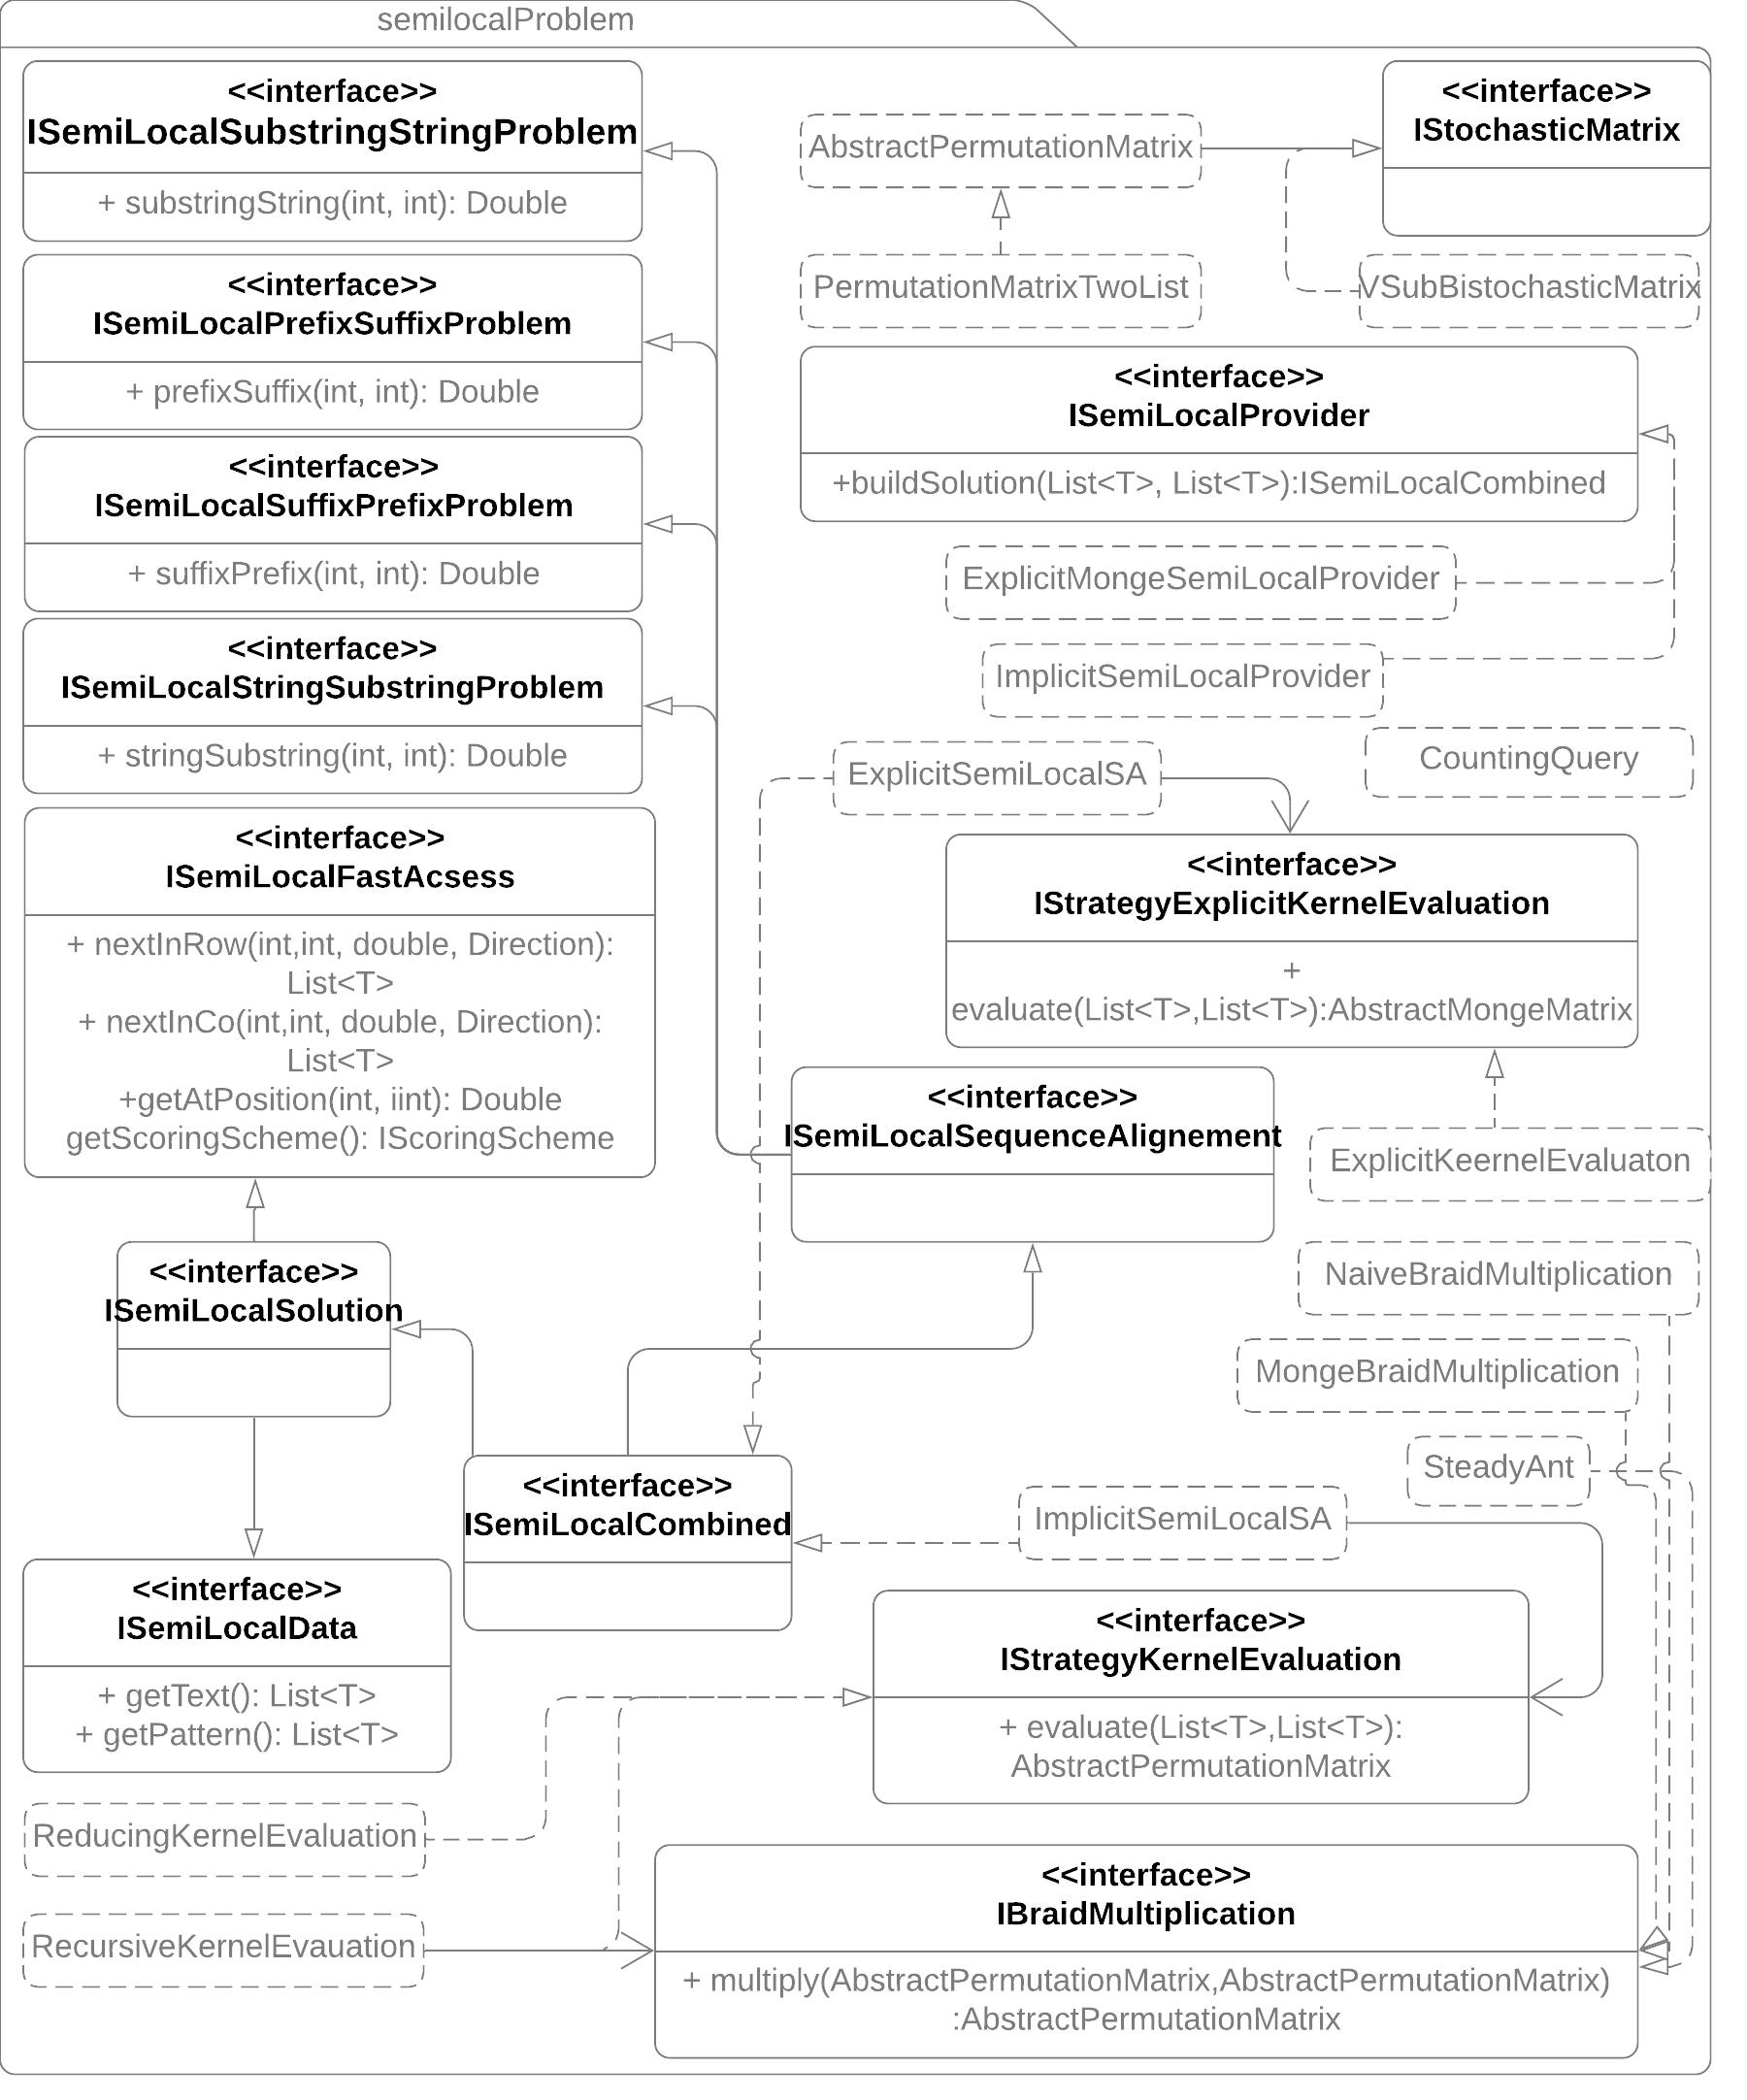
\includegraphics[height=0.72\columnwidth,angle=90]{Mishin/figures/Library.png}
  \caption{Диаграмма классов UML части библиотеки, относящейся к различным задачам, основанным на  semi-local задачах; Часть деталей и классов опущена}\label{fig:libraryProblem}
\end{figure}

\new{Если необходим константный доступ к произвольным элементам матрицы, то можно воспользоваться классом \emph{ExplicitSemiLocalSA}, который хранит матрицу $H_{a,b}$ в явном виде.}

\todo{нет перехода}\emph{ExplicitSemiLocalSA} хранит матрицу $H_{a,b}$ в явном виде.
В данном случае нет экономии памяти, но доступ к произвольному элементу матрицы константный $O(1)$. 
\new{В качестве алгоритма решения непосредственно используется алгоритм \ref{alg:monge} с использованием алгоритма \emph{smawk}~\cite{aggarwal1987geometric} в качестве операции $\otimes$. }
Для решения задачи semi-local используется алгоритм \emph{smawk}~\cite{aggarwal1987geometric}, \todo{что это значит? не уловил}отвечающий операции  $\otimes$.

% Стоит отметить, что недавние исследования~\cite{gawrychowski2020submatrix}, позволяют добиться 
% Нужно ли описать scorinSCheme



% \emph{ISemiLocalProvider}, \emph{ISemiLocalCombined} === паттерн фабричный метод
% набор классов и интерфейсов связанных с \emph{}
% Strategy --- стратегия


\subsubsection{Модуль semilocalApplication.}
В данном модуле реализованы алгоритмы\footnote{Детальное описание алгоритмов и их доказательств можно найти в~\cite{tiskin2006all}.}, для решения следующих задач:
\begin{enumerate}
    \item \emph{CompleteAMatch},
    \item \emph{Minimal-inclusive ThresholdAMatch},
    \item \emph{WindowAMatch},
    \item \emph{WindowSubstring},
    \item \emph{FragmentSubstring},
    \item \emph{BoundedLengthSmithWatermanAlignment}.
\end{enumerate}

Первая задача относится к нахождению значения максимального выравнивания заданного шаблона $p$ и всех префиксов текста $t$ из всевозможных суффиксов из данного префикса:
\todo{что за h[j] здесь? --- из текста не ясно --- в формуле же j пробегает от 0 до t + префикс}
\begin{equation}
    d[j] = \max _{i \in 0 ..j} SA(p,t[i,j]), j \in 0..|t|.
\end{equation}

В рамках второй задачи ставится задача нахождения всех непересекающихся повторов шаблона $p$ в тексте $t$, чьи длины минимальны, а значение выравнивания выше заданного порога подобия $h$\todo{h перегружено, теперь не перегружено:)}.

В третьей задаче необходимо найти все подстроки текста $t$ длины $w$, чьё выравнивание с шаблоном $p$ больше заданного порога подобия $h$. Заметим, что искомы подстроки могут пересекаться.

Все эти три задачи сводятся к анализу подматрицы задачи semi-local, отвечающей подзадаче srting-substring.
В зависимости от выбранного алгоритма решения задачи semi-local, его асимптотическая сложность будет равна $O(n \times m \times \log n)$ или $O(v \times  m \times n)$.

\begin{figure}
    \centering
    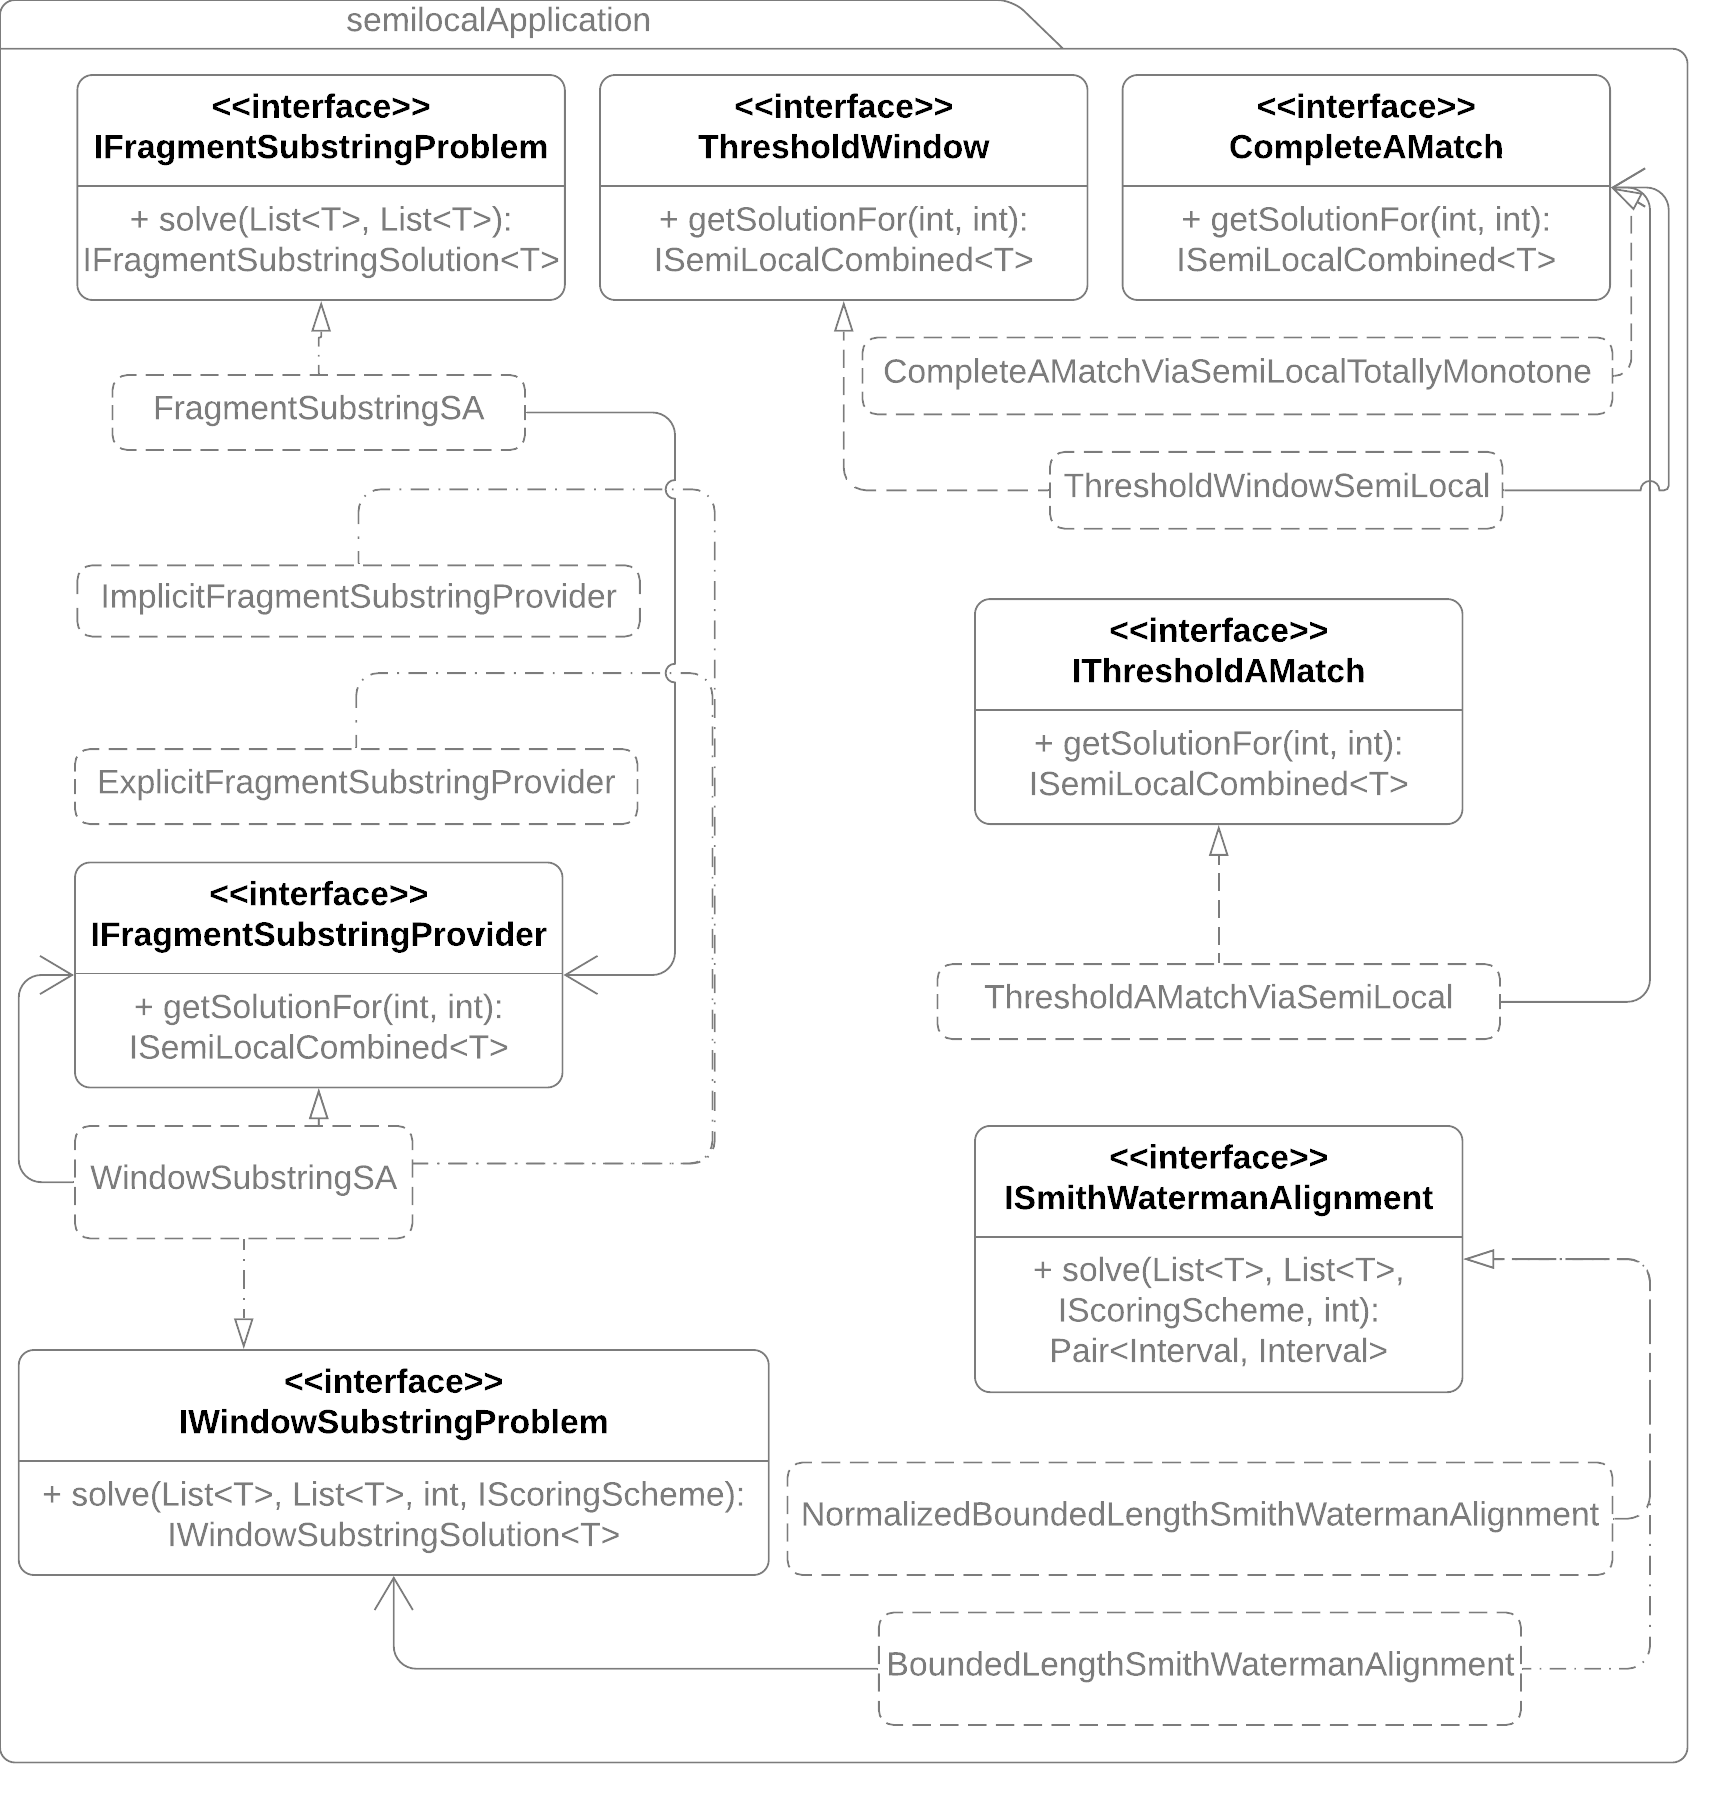
\includegraphics[width=1.35\columnwidth,angle=90]{Mishin/figures/semiLocalApplication.png}
    \caption{Диаграмма классов UML части библиотеки, относящейся к semi-local задачам. Часть деталей и классов опущена}\label{fig:libraryApplication}
\end{figure}

Задача FragmentSubstring формулируется следующим образом: для заданного множества интервалов (подстрок) $r$ из текста $t$ размера $m$ и текста $b$ размера $n$ необходимо вычислить semi-local матрицу для каждого фрагмента из $r$ против $b$.
Алгоритмы решения имеют асимптотическую сложность $O(v^2 \times r \times  n \times \log m \times \log mv)$\footnote{Существует возможность улучшить асиптотику до $O(v \times r \times  n \times \log^{2} m)$.} и $O(r \times n \times m  \times \log m)$.

Задача WindowSubstring является частным случаем  FragmentSubstring, в которой размер фрагментов фиксирован.
Асимптотическая сложность решения уже будет $O(n \times m \times \log n)$ и $O(v^2 \times  m \times n)$.

Обе задачи основаны на двоичном разложении числа и предподсчете semi-local решений, отвечающих данным разложениям.

Задача SmithWatermanAlignment относится к задаче локального выравнивания строк.
В рамках данной задачи необходимо вычислить значение максимального локального выравнивания между строками $a$ и $b$, т.е. найти пару подстрок, на которых достигается максимальное выравнивание.
Зачастую данная задача представляет интерес при наложении различных дополнительных ограничений~\cite{arslan2004dynamic}.
Примером такого ограничения является ограничение минимальной длинны подстрок.
Данное ограничение реализовано с помощью алгоритма из~\cite{tiskin2019bounded} и инкапсулировано в соответствующем классе BoundedLengthSmithWatermanAlignment.
% Нетрудно заметить, что часть алгоритмов в той или иной степени может быть адаптирована к задачам поиска повторов в документации.
% Для задачи поиска по образцу такими кандидатами являются алгоритмы для решения задачи \emph{Minimal-inclusive ThresholdAMatch} и \emph{WindowSubstring}.
% Для задачи поиска групп повторов могут быть применены  алгоритмы для \emph{WindowAMatch},
% \emph{Minimal-inclusive ThresholdAMatch}, \emph{BoundedLengthSmithWatermanAlignment} и \emph{semi-local}.

% Адаптация алгоритмов к поиску повторов описана в следующем разделе.
% Экспериментальная проверка асимптотики части алгоритмов, а так же их потенциальная возможность применения к большим данным даны в главе~\ref{appob}.

% Соответствующая адаптация части алгоритмов описана в следующем разделе.


\section{Приложение для поиска повторов в документации ПО}\label{searchPO}
В данной главе представлено приложение для поиска повторов в документации ПО, в рамках которого будет производится экспериментальное исследование применимости алгоритмов, решающих полулокальные задачи поиска.
Также описаны основные технические решения и архитектура приложения.
Описаны подходы для поиска текстовых повторов.
Для каждой из задач поиска повторов описано решение, основанное на использовании библиотеки алгоритмов для полулокальных задач (см. главу~\ref{librarySection}).

% Реализация приложения для поиска повторов в JavaDoc докумен-тации с применением алгоритмов решения полулокальных задач


\subsection{Общая архитектура приложения}
На рисунке~\ref{fig:application} представлена архитектура приложения.
Оно реализовано в виде двух крупных компонент.

\begin{figure}[H]
    \includegraphics[width=\columnwidth]{Mishin/figures/arhitecture.png}
    \caption{Диаграмма компонентов системы}\label{fig:application}
\end{figure}


Первая компонента (клиентская часть)~--- это пользовательский интерфейс (\emph{UI}), который отвечает за визуализацию и взаимодействие с пользователем.
Пользователь настраивает параметры поиска повторов, тип поиска, указывает файлы, в которых необходимо произвести анализ на дубликаты, или путь к проекту на Github в сети Интернет (см. Рис.~\ref{fig:startApp}).
Клиентская часть реализована на языках \textsc{Python} и \textsc{Java Script}.
Детальное описание клиентской части приведено в разделе~\ref{clinet}.

Вторая компонента (серверная часть) отвечает за поиск повторов согласно заданным настройкам.
Данная компонента реализована на языке \textsc{Kotlin}.
В разделе~\ref{server} детально описана её функциональность.

Взаимодействие между компонентами осуществляется посредством \textsc{JSON}-формата.
Приложение реализовано в виде вэб-приложения, которое запускается в докер-контейнере, что минимизирует пользовательские требования для запуска программы\footnote{Для запуска приложения на ПК достаточно иметь установленные \textsc{Docker} и вэб-браузер.}.

Стоит отметить, что в этой работе сделан основной акцент на поиск повторов в \textsc{JavaDoc} документации в силу её актуальности для данного \todo{какого формата??}\new{удалить текст после докумнетации. Оставить реф  }формата (см. раздел~\ref{duplicateReport}).

\begin{figure}[h!]
    \centering
    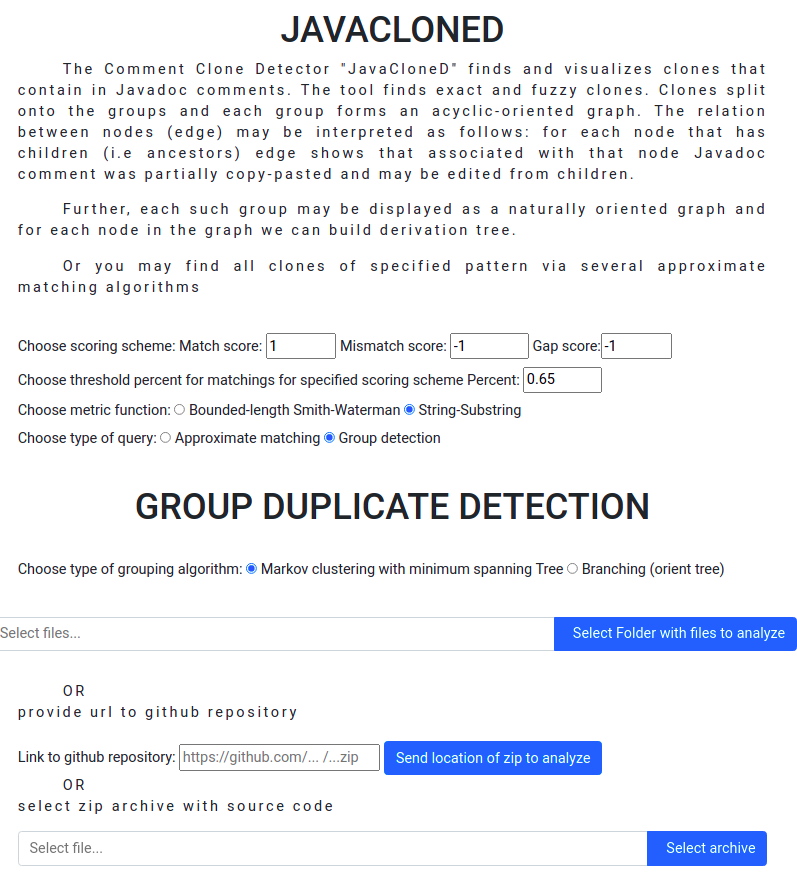
\includegraphics[width=1.3\columnwidth,angle=90]{Mishin/figures/startApp.png}
    \caption{Интерфейс пользователя перед запуском анализатора для случая поиска групп повторов}\label{fig:startApp}
\end{figure}

\subsection{Клиентская часть}\label{clinet}
Как было отмечено выше, клиентская часть реализована в виде вэб-приложения, которое написано посредством \textsc{python}-фреймворка \textsc{flask}\footnote{\url{https://flask.palletsprojects.com/en/1.1.x/}~--- микро-фреймворк для написания вэб-приложений.}.
На основной странице вэб-приложения пользователь выставляет тип решаемой задачи, параметры запуска, указывает исходные файлы и запускает вычисления.
Пользователь имеет возможность выбрать одну из задач: \emph{``Поиск повтора по шаблону''} или \emph{``Поиск всех групп повторов''}.

Для визуализации найденных повторов в случае с  ``Поиском повтора по шаблону'' результаты отображаются на странице ответа с цветовой расцветкой.
% \begin{figure}[h!]
%     \centering
%     \includegraphics[width=0.5\columnwidth]{Mishin/figures/outputExampleAmatch.png}
%     \caption{Визуализация найденных повторов для поиска по шаблону}\label{fig:pattViz}
% \end{figure}
Для групп повторов механизм визуализации более комплексный (см. рис~\ref{fig:groupViz}): используется три окна для интерпретации результатов.

\begin{figure}[h!]
    \centering
    \includegraphics[width=\columnwidth]{Mishin/figures/outputGroup.png}
    \caption{Визуализация групп повторов}\label{fig:groupViz}
\end{figure}


\new{В первом окне визуализируется отношение ``наследования'' между повторами.}
Первое окно отвечает за \todo{надо переформулировать} отображение отношений между фрагментами, которые состоят в отношении (имеют похожие части).
\todo{дети и роджители из ниоткуда. Вроде предложение с наследованием решает проблему}
Интерпретация следующая: для текущего узла ``родителем'' являются все те фрагменты, в которые была взята часть информации с текущего фрагмента и, возможно, видоизменена.
``Детьми'' являются те фрагменты, c которых, вероятнее всего, произошло дублирование информации.

Второе окно отвечает за представление каждого повтора в виде иерархической структуры.
Представление реализовано в виде \emph{tree control}~--- для каждого повтора (вершины) строится ориентированное дерево вывода из этой вершины.
Такая интерпретация показывает, откуда вероятнее всего ``произошел повтор'', т.е. откуда произошло дублирование данных.

Третье окно отвечает за визуализацию соответствующей группы повторов в виде ориентированного графа.
Это позволяет увидеть структуру найденной группы.
Все три окна синхронизированы между собой.

Описание используемых алгоритмов для нахождения повторов даны в разделах~\ref{fics} и~\ref{grouppa} соответственно.


\subsection{Серверная часть}\label{server}
Как было указано выше, эта часть приложения отвечает за реализацию поиска повторов в документации.

На Рис.~\ref{fig:application} выделены компоненты серверной части (\emph{Kotlin application}).
Общий подход поиска повторов заключается в следующем.
Сперва происходит синтаксический анализ с целью нахождения тех фрагментов, которые будут анализироваться согласно выбранным параметрам, заданными пользователем.
В данной работе анализируются \textsc{JavaDoc} документация, а именно \textsc{JavaDoc}-комментарии методов, классов и интерфейсов.
Это осуществлено с использованием библиотеки \textsc{JavaParser}\footnote{\url{https://javaparser.org/}.}.
Для анализа иного вида документации, например, обычный текст, как в случае с поиском по образцу, достаточно в модуле Parser реализовать необходимые интерфейсы.
Далее, комментарии обрабатываются различными фильтрами: происходит токенизация, лемматизация, убираются стоп-слова и пр.
\new{Для препроцессинга текстовых фрагментов используется фреймворк \emph{core nlp}\footnote{\url{https://stanfordnlp.github.io/CoreNLP/}}}
\todo{переформулировать} Данная обработка происходит с частичным использованием функциональности стэнфордского фреймворка \emph{core nlp}\footnote{\url{https://stanfordnlp.github.io/CoreNLP/}} для обработки естественного языка.
После этапа предобработки фрагментов происходит конвертация слов в промежуточное представление в виде чисел с целью экономии памяти и ускорения работы алгоритмов.
Затем происходит запуск соответствующих алгоритмов поиска, о которых пойдет речь дальше.


\subsection{Алгоритмы для решения задачи поиска повторов}\label{fics}

В данном разделе описаны алгоритмы для решения задачи поиска по образцу, \todo{э? какой моделью?} согласующиеся с определенной моделью в главе~\ref{Model}\new{просто убрать}.
Алгоритмы реализованы с помощью разработанной библиотеки алгоритмов (см. главу~\ref{librarySection}).

\subsubsection{Улучшенный алгоритм интерактивного поиска.}
В данном разделе описана улучшенная версия алгоритма из~\cite{luciv2019interactive}.
Псевдокод алгоритма представлен ниже (Algorithm~\ref{alg:patternMathing1}).

\begin{algorithm}[t!]
\caption{Нечеткий поиск по шаблону с использованием semi-local}\label{alg:patternMathing1}
Вход: шаблона поиска $p$, текст $t$, пороговое значение подобия $k$\\
Выход: множество непересекающихся повторов шаблона $p$\\
Комментарии:
\begin{equation}
    k_{di}=|p|*(\frac{1}{k}+1)(1-k^2)
\end{equation}
Псевдокод:
\begin{algorithmic}[1]
\State $W = semilocalsa(p,t)$\Comment{1 фаза}
\State $ H^{str-sub}_{p,t} =  W.stringSubstringMatrix()$
\State $ M[j,i] = H^{str-sub}_{p,t}[i,j] $
\State $lstW = queryWindows()$\Comment{2 фаза}
\State $W_2 = processDiagonal()$
\State $W_3 = UNIQUE(W_2)$\Comment{3 фаза без изменений}
\For{$w \in W_3$}
\If{$\exists w^{'} \in W_3:w \subset w^{'} $}
\State $remove$ $w$ $from$ $W_3$
\EndIf
\EndFor
\State $return$ $W_3$

\end{algorithmic}
\end{algorithm}

\begin{figure}[t!]
\centering
    \includegraphics[width=0.5\columnwidth]{Mishin/figures/M2.png}
    \caption{Пример обхода матрицы $M$. Трапеция соответствует всем подстрокам текста, чья длина ограничена интервалом $I$. Треугольники отвечают скользящим окнам.
    Обход происходит с конца текста.
    }\label{passage}
\end{figure}

В строках 1--3 вычисляется решение задачи semi-local SA, в частности, подзадачи string-substring, а также происходит операция транспонирования, полученной матрицы, для получения матрицы $M$.
Далее в строке 4 для каждого окна размера $L_{w}$ вычисляется значение выравнивания с шаблоном $p$, и результат сохраняется в список $lstW$.
После этого обрабатывается трапеция в матрице $M$, которой отвечают все подстроки текста $t$ с размером из интервала $I=[|p|k,\frac{|p|}{k}]$.
Она обходится таким образом, что в результате внутри каждого окна размера $L_{w}$, чья  мера подобия выше заданного порога $-k_{di}$, находится подстрока с длиной из интервала $I$, которая максимально похожа на образец.
Если таких подстрок несколько, будет выбираться наиболее длинная (строка 5).
Далее результат сохраняется в множество $W_{2}$.
Пример обхода представлен на Рис.~\ref{passage}.

\paragraph*{Корректность алгоритма}\mbox{}

Нетрудно заметить, что представленная версия алгоритма имеет лучшую асимптотическую сложность, чем исходный алгоритм.
Более того, все свойства алгоритма сохраняются.
Исходный алгоритм разбит на три фазы: ``сканирование'', ``усушка'' и ``фильтрация''.

В первой фазе исходный текст $t$ анализируется скользящим окном размером $w_{s} = \frac{|p|}{k}$, где $k \in [\frac{1}{\sqrt{3}},1]$ параметр алгоритма, с шагом в один символ, а именно вычисляется редакционного расстояние\footnote{Метрика, минимальное количество операций вставки, удаления и замены одного символа на другой для превращения одной строки в другую.} между каждым окном и заданным шаблоном $p$.
Согласно~\cite{luciv2019interactive} асимптотическая сложность данного шага $O(|p|^2 \times |t|)$.

Заметим, что редакционное расстояние может быть выражено через выравнивание последовательностей.
Конкретнее, редакционное расстояние для данного случая выражается через следующую схему оценки:
\begin{equation}\label{weightAppr}
    (w_{+},w_{0},w_{-}) = (0,-2,-1).
\end{equation}
Соответственно, редакционное расстояние можно заменить на выравнивание последовательностей с весами $(0,-2,-1)$ и искать максимальное выравнивание без потери свойств алгоритма в силу эквивалентности двух задач.
Из этого следует, что можно применить алгоритмы для решения semi-local SA.
В силу формулы~(\ref{weightNormalization}), значение нормализованной схемы будет следующее:
\begin{equation}
    (0, -2, -1) \rightarrow (1,\frac{\mu=0}{v=1}, 0).
\end{equation}
Таким образом, используя нормализацию, задачу можно свести к semi-local LCS.
А, следовательно, асимптотическая сложность первой фазы алгоритма из~\cite{luciv2019interactive} может быть улучшена до $O(|t| \times |p|)$ вместо $O(|t| \times |p|^2)$.
Данная стадия эмулируется в строке 1 представленного алгоритма.

Во второй фазе происходит так называемая ``усушка''~--- для каждого окна происходит вычисление максимальной подстроки, на которой достигается минимальное значение редакционного расстояния (в случае выравнивания последовательностей это относится к максимальному значению).
При равенстве расстояний выбирается подстрока наибольшая по длине из интервала $I$.
Асимптотическая сложность данной фазы оценивается как $O(|t| \times |p|^4$).

Для улучшения данной фазы применяется следующее.
Матрица решений $H_{p,t}$ содержит подматрицу string-substring ($H^{str-sub}_{p,t}$), которая содержит значения выравнивания шаблона $p$ со всеми подстроками текста $t$.
После применения операции транспонирования к матрице $H^{str-sub}_{p,t}$ получается матрица $M$, в которой присутствует трапеция, которая отвечает всем подстрокам текста $t$ с длиной из интервала $I$ (Рис.~\ref{passage}).
Алгоритм обхода представлен на Рис.~\ref{passage}.
В силу того, что во время обхода посещаются смежные ячейки, асимптотическая сложность доступа к матрице $O(1)$, согласно~\cite{tiskin2008semi}.
Всего будет посещено $O((\frac{|p|}{k}-|p|k)*|t|)=O(|p|\times|t|)$ ячеек.
В рамках обхода мы будем поддерживать список $rowMax$ из $O(p)$ элементов, в котором будут содержаться наибольшие подстроки с максимальным выравниванием для текущих префиксов (отвечает строкам, черный треугольник на Рис.~\ref{passage}).
При очередном проходе столбца в трапеции мы обновим максимумы для строк (текущее обозреваемое окно, треугольник) с учетом сдвига на единицу (последняя строка уходит, появляется новая из одного элемента~--- на Рис.~\ref{passage} после сдвига по диагонали добавится строка, а снизу удалится строка полностью).
Далее мы проверяем, что значение выравнивания окна размером $L_{w}$ выше порога $-k_{di}$, отвечающее текущему треугольнику.
Для этого мы просто проверяем элемент списка $lstW$, отвечающий этому окну.
Если значение выше порогового, тогда наиболее длинная подстрока с максимальным выравниванием сохраняется в множество $W_{2}$.
Соответственно, асимптотическая сложность обработки каждого столбца (каждого треугольника) $O(|p|)$.
Таких столбцов $|t|$ штук.
Таким образом, асимптотическая сложность всей второй фазы $O(|t| \times |p|)$, а все свойства исходного алгоритма сохранены.

Третья фаза, отвечающая за фильтрацию фрагментов, остается без изменений.
Её асимптотическая сложность оценивается как $O(|p| \times \log |p|)$, согласно~\cite{luciv2019interactive}.

Таким образом, предложенный алгоритм сохраняет все свойства сиходного и имеет асимптотическую сложность $O(|p| \times |t|)$.


\subsubsection{Алгоритм нечеткого поиска шаблона с использованием ThresholdAMatch.}
\new{Следующее решение относится к использованию алгоритма~\ref{alg:patternMathing2}, реализация которого уже содержится в библиотеке алгоритмов.}
Более простое решение \todo{кеажется, надо переформулировать} относится к алгоритму~\ref{alg:patternMathing2}, реализация которого уже содержится в библиотеке алгоритмов. 
Он позволяет найти все непересекающиеся повторы шаблона $p$ в тексте $t$.

Сперва решается задача \emph{CompleteAMatch}, в рамках которой для каждого столбца $j$ подматрицы string-substring находится максимальное значение и позиция $(i,j')$, в которой оно достигается, т.е. находится суффикс префикса, который больше всего похож на шаблон.
Далее, над полученным результатом производится фильтрация, начиная с конца.
В результате чего остаются только непересекающиеся повторы минимальной длины, которые больше заданного порога подобия.
Асимптотическая сложность данного решения зависит от выбранного алгоритма решения semi-local и оценивается как  $O(|t| \times |p| \times \log |t|)$, $O(|t| \times |p| \times v^2)$ или $O(|t| \times |p| \times v)$, 
соответственно.
Данный алгоритм рассматривается как альтернатива алгоритму~\ref{alg:patternMathing1}.

\begin{algorithm}[b!]
\caption{Нечеткий поиск по шаблону с использованием Min-inclusive ThresholdAMatch}\label{alg:patternMathing2}
Вход: шаблона поиска $p$, текст $t$, пороговое значение меры подобия $h$\\
Выход: множество непересекающихся повторов шаблона $p$\\
Псевдокод:
\begin{algorithmic}[1]
\State $maxSuffixes= CompleteAMatch(p,t)$
\State $reverse(maxSuffixes)$
\State $result = \emptyset$
\For{$(i,j,score) \in maxSuffixes$}
   \If{$score \geq h \& j \leq res.last().i $} 
    \State $res.add((i,j,score))$ 
    \EndIf
\EndFor
\State $return$ $result$

\end{algorithmic}
\end{algorithm}

% \subsubsection{Алгоритм нечеткого поиска шаблона с использованием Разреза}

% Еще одним решением на основе \emph{semi-local} является следующий алгоритм.
% Во-первых, задачу поиска по шаблону можно сформулировать с иной точки зрения: 
% необходимо найти все максимальные по выравниванию непересекающиеся повторы шаблона $p$ в тексте $t$, т.е получить такую цепочку непересекающихся интервалов $(i_1,j_1),...,(i_n,j_n)$, что на $(i_k,j_k)$ достигается максимальная похожесть на еще непокрытой найденными интервалами части текста $t$.
% В рамках задач \emph{semi-local} это означает разбитие матрицы \emph{string-substring} на непересекающиеся подматрицы, с учетом максимумов в подматрицах.
% Последнее относится к быстрому поиску максимума в матрице (\emph{range maximum query}).
% В силу того, что матрица \emph{string-substring} является матрицей Монжа, можно применить результат из статьи ~\cite{gawrychowski2020submatrix}. 
% Для этого необходимо реализовать структуру данных, асимптотическая сложность построения которой равна $O(|t|\times \log |t|)$ (размер структуры выражается как $O(|t|)$), которая позволяет делать запросы на поиск максимума в произвольной подматрице, имеющие асимптотическую сложность $O(\log \log|t|)$.
% Учитывая, что непересекающихся повторов в тексте $t$ может быть в худшем случае $|t|$ штук,
% для их нахождения необходимо осуществить $|t|$ запросов на поиск максимуму.
% Следовательно, конечная асимптотика алгоритма $O(|t| \times \log \log t) +O($\emph{сложность подсчета 
% semi-local}$)=O($\emph{сложность подсчета 
% semi-local}$)$, так как $\log \log |t| \leq |p|$ для достаточно больших значений $|t|$. 
% Псевдокод алгоритма представлен на листинге~\ref{alg:patternMathing3}.

% \begin{algorithm}[h]
% \caption{Нечеткий поиск по шаблону с использованием maxRangeQuery}\label{alg:patternMathing3}
% Вход: шаблон поиска $p$, текст $t$, пороговое значение похожести $h$\\
% Выход: множество непересекающихся повторов шаблона $p$\\
% Комментарии: в реализации $h$ высчитывается исходя из схемы оценки и процента похожести, выраженного через число из отрезка $[0,1]$\\
% Псевдокод:
% \begin{algorithmic}[1]
% \State $S = SolveSemiLocalSA(p,t)$
% \State $W = BuildStructForRangeQuery(S)$
% \State $IntervalsToSearch = \emptyset $
% \State$IntervalsToSearch.add((0,|t|))$
% \State $result = \emptyset$
% \While{$IntervalsToSearch.isNotEmpty()$}
%     \State $(i,j) = IntervalsToSearch.pop()$
%     \State $score,i^{'},j^{'} = W.query(i,j)$
%     \If{$score \geq h $} 
%     \State $result.add(( i^{'},j^{'},score ))$
%     \State $IntervalsToSearch.add(i,i^{'})$        \State $IntervalsToSearch.add(j^{'},j)$
%     \EndIf
% \EndWhile
% \State $return$ $result$

% \end{algorithmic}
% \end{algorithm}


% Для апробации применимости \emph{semi-local} было решено реализовать алгоритм~\ref{alg:patternMathing2} т.к
% для~\ref{alg:patternMathing1} была произведена апробация в статье~\cite{luciv2019interactive}, а~\ref{alg:patternMathing3} на данный момент не имеет доказанных теоретических свойств и требует использования сложной структуры данных из~\cite{gawrychowski2020submatrix}.

% Для задачи поиска по образцу постпроцессинг не нужен.

\subsection{Алгоритмы для решения задачи поиска групп повторов}\label{grouppa}
В данном разделе описаны алгоритмы решения задачи поиска групп повторов на основе использования библиотеки алгоритмов и применения графовых алгоритмов.

Согласно определенной в секции~\ref{Model} модели, для решения задачи поиска групп повторов необходимо
задать функцию $g$, которая измеряет меру подобия двух фрагментов, и выбрать предикат $\gamma$.
Заметим, что для рассматриваемого случая, текстовыми фрагментами, в которых ищутся повторы, являются цельные \textsc{JavaDoc}-комментарии.
Соответственно, в данной работе \todo{в отношении}\new{повторами будут служить семантически замкнутые  фрагменты текста, как и в~\cite{soto2015similarity}.} поиска групп повторов повторами будут служить семантически замкнутые куски текста, как и в~\cite{soto2015similarity}\footnote{В~\cite{soto2015similarity} это были топики текста в \textsc{Dita} документации.}, т.е. \textsc{JavaDoc} комментарии.

Весь набор комментариев образует граф.
Он может быть как ориентированным, так и неориентированным.
Это зависит  от того, является ли $g$ симметричной по отношению к своим аргументам.
Таким образом, в полученном графе можно выделить группы повторов согласно предикату $\gamma$.
На~\ref{alg:groupDuplicate} представлен псевдокод алгоритма.
Отметим, что асимптотическая сложность алгоритма выражается как $\max (O(|t|^2*g), O(s))$.

Функция $g$ может быть определена через локальное, полулокальное и глобальное выравнивание, соответственно.
В данной работе в качестве $g$ выбраны следующие алгоритмы из библиотеки алгоритмов:
\begin{itemize}
    \item BoundedLengthSmithWaterman~--- локальное выравнивание,
    % , симметричная функция.
    \item Semi-local SA~--- полулокальное выравнивание.
    % не симметричная функция.
    % \item \emph{ThrehsoldAMatch} --- поиск по шаблону. 
\end{itemize}

\begin{algorithm}[t!]
\caption{Алгоритм поиска групп повторов для JavaDoc-комментариев}\label{alg:groupDuplicate}
Вход: набор комментариев $t_{i}$, функция $g$, которая измеряет меру подобия между двумя комментариями, функция $s$, которая согласно выбранному предикату $\gamma$ строит группы, пороговое значение меры похожести $h$\\
Выход: группы непересекающихся повторов\\
Псевдокод:
\begin{algorithmic}[1]
\State $graph = Graph(vertices=t)$
\For{$t_{i} \in t $}
\For{$t_{j} \in t,t_{i} \neq t_{j} $}
\If{$g(t_{i},t_{j})\geq h $}
\State $addEdge(t_{i},t_{j},g(t_{i},t_{j}))$
\EndIf
\If{$g(t_{j},t_{i}) \geq h$}
\State $addEdge(t_{j},t_{i},g(t_{j},t_{i}))$
\EndIf
\EndFor
\EndFor
\State $groups = s(graph)$
\State $return$ $groups$
\end{algorithmic}
\end{algorithm}

% На~\ref{1,2,3} представлены алгоритмы, определяющие функцию $s$

Следующие эвристические соображения помогают определить функции $s$, которые подходят для нахождения групп.

Во-первых, в силу того, что мы рассматриваем граф, естественным образом задача сводится к кластеризации графа~--- выделению компонент (сильной) связности.

Во-вторых, ориентированное ребро $a \xrightarrow{g(a,b)} b$ в графе можно естественным образом интерпретировать так: часть текста из $b$ была скопирована в фрагмент $a$ или текст $b$ был скопирован, и в новом фрагменте произведена модификация этой копии и получено $a$.
При существовании обратного ребра будем считать, что при условии $g(a,b)\geq g(b,a)$, $a$ является потомком $b$ (помним, что в общем случае $g(a,b)\neq g(b,a)$ и наоборот.

В-третьих, очень часто бывает, что повторы практически не отличаются друг от друга или же в точности совпадают друг с другом.
Такие повторы хочется отличать от обычных.
Если рассматривать граф, такое состояние для части вершины выражается через термин \emph{клика}\footnote{Полный граф на заданных вершинах.} и относится к задаче поиска клики.
Соответственно, новый граф, в котором присутствуют клики, строится из исходного обновлением весов тех ребер, которые входят в клики или находятся внутри клик.

В-четвертых, ассоциированный с группой ориентированный граф должен быть деревом.
Эта эвристика основана на том, что вершина не может быть потомком сама себе (наличие циклов) и не может иметь двух одинаковых потомков (проблема множественного наследования).
Иными словами, граф должен являться деревом.

Исходя из описанных выше эвристик, были разработаны алгоритмы~\ref{alg:cluster1},~\ref{alg:clusterMcl}.
Также применён алгоритм из статьи~\cite{tofigh2009optimum}.

В~\ref{alg:cluster1} используется идея иерархической кластеризации с тем изменением, что добавляется новый вид вершины, который олицетворяет клики.
Как известно, поиск клики~--- это \emph{NP}-полная задача.
Поэтому в данном алгоритме произведена аппроксимация поиска клик: листовая вершина принадлежит кластерному узлу, если её расстояние до клики больше заданного порога меры подобия для клик.
% \red{Для подсчета расстояний будет использоваться \emph{минимальное расстояние между вершинами}.} 
% Существует разные варианты подсчета расстояний, о них подробно  будет описано в главе TODOапробации.
В ходе алгоритма в цикле while происходит нахождение двух ближайших вершин согласно выбранной метрике, их объединение согласно правилам и пересчет матрицы расстояний, которая отвечает уже новому графу.
В общем случае\footnote{Некоторые метрики позволяют считать асимптотически быстрее.} пересчет матрицы требует $O(n^2)$ времени, где $n$~--- количество вершин.
В худшем случае  цикл while будет исполняться $O(n)$ раз,
тогда асимптотика алгоритма составит $O(n^3)$.
% песос пример нужен лучше напиши епта

% иерархичпская кластеризация
\begin{algorithm}[t!]
\caption{Алгоритм выделения групп на основе Иерархической кластеризации}\label{alg:cluster1}
Вход: граф $G$ с матрицей расстояний, функция  $f$, которая считает дистанцию между вершинами, пороговое значение меры подобия $h_{clique}$, при котором вершины образуют очередной уровень в иерархии, $h_{group}$~--- пороговое значение меры подобия\\
Выход: иерархические группы повторов \\
Псевдокод:
\begin{algorithmic}[1]
\State $roots = G.vertices()$
\While{$roots.isNotEmpty()$}
\State $(from, to,score) = closestVertices(root)$
\State $newVertex = switch \{$
\State $score\geq h_{clique} , from,to \in Leaf \rightarrow Clique(from,to) $
\State $score\geq h_{clique} , to \in Clique,from \in Leaf \rightarrow to.add(from);to $
\State $score\geq h_{clique} , from,to \in Clique \rightarrow from.addAll(to);from$
\State $score\geq h_{group}, \rightarrow ClusterNode(from,to) $
\State $else \rightarrow break$ 
\State $\}$
\State $G.recalcualateDistance()$
\State $roots.remove(from)$
\State $roots.remove(to)$
\State $roots.add(newVertex)$
\EndWhile
\State $return$ $roots$
\end{algorithmic}
\end{algorithm}

В алгоритме~\ref{alg:clusterMcl} использована идея кластеризации на основе марковских моделей~\cite{dongen2000cluster} и дальнейшего построения минимальных остовных деревьев внутри каждого кластера.
Асимптотическая сложность первого шага реализации в данной работе оценивается как $O(n^3)$ в худшем случае.
Нахождение минимального остовного дерева реализовано с помощью алгоритма Крускала с использованием системы непересекающихся множеств.
Сложность второго шага~--- $O(n^2 \times \log n)$.
Таким образом, общая сложность оценивается как $O(n^3)$.

% mcl clustering
\begin{algorithm}[t!]
\caption{Алгоритм выделения групп на основе Марковских моделей}\label{alg:clusterMcl}
Вход: граф $G$ с матрицей расстояний\\
Выход: группы повторов с структурой группы в виде дерева\\
Псевдокод:
\begin{algorithmic}[1]
\State $trees = \emptyset$
\State $ clusters = mclClustering(G)$
\For{$cluster \in clusters$}
\State $tree =  BuildMaximumSpanningTree()$
\State $trees.add(tree)$
\EndFor
\State
\State $return$ $trees$
\end{algorithmic}
\end{algorithm}

Алгоритм~\cite{tofigh2009optimum} решает задачу построения такого ориентированного подграфа $G_{branch}$ из исходного $G$, такого что:
\begin{itemize}
    \item в нем нет циклов,
    \item ни в какую вершину не входит больше одного ребра.
\end{itemize}
Причем среди всех таких подграфов он оптимален:
\begin{equation}
\sum_{w \in G_{branch}} w \geq \sum_{w^{'} \in G_{branch^{'}}} w^{'}.
% \forall G_{branch^{'}} 
\end{equation}
Это соотносится с последней эвристикой о том, что граф должен быть деревом.
Алгоритм из~\cite{tofigh2009optimum} обладает асимптотической сложностью $O(n^2)$.

% вероятностная кластеризация
% разбить компоненты сильной связности-> построить ориентированное дерево
%  

%\vspace{10 mm}
Результаты применимости описанных алгоритмов из  данной главы к поиску повторов в документации ПО представлены в главе~\ref{appob}.


\section{Апробация и анализ результатов}\label{appob}
В данной главе представлены результаты апробации алгоритмов из библиотеки алгоритмов полулокальных задач.
Также дана оценка применимости решений полулокальных задач semi-local LCS и SA к задаче поиска групп повторов в \textsc{JavaDoc}-комментариях.


\subsection{Тестовый стенд}

Для проведения экспериментов использовалась машина с процессором Intel-Core i5 и оперативной памятью размера 16GB, операционной системой Ubuntu 18.04 Bionic.
На каждый запуск jar-файла выделялось 10GB памяти.

\subsection{Экспериментальная проверка асимптотики}

В данном разделе описаны экспериментальные результаты запусков части алгоритмов из реализованной библиотеки алгоритмов (см. главу~\ref{librarySection}) и приведена их интерпретация.

На Рис.~\ref{fig:speedlcs} представлен результат запусков обычного prefix LCS (\emph{prefix lcs}), prefix LCS с хранением результатов с помощью одной строки (\emph{light-prefix lcs}) и semi-local LCS (\emph{semi-local lcs reducing}).
Исходя из результатов, можно сделать вывод, что скорость вычисления semi-local LCS сопоставима с вычислением обычного prefix LCS.

\begin{figure}[t!]
\centering
    \includegraphics[width=0.8\columnwidth]{Mishin/figures/semiLocalvsPrefixLCS.png}
    \caption{Результат запусков различных версий подсчета LCS }\label{fig:speedlcs}
\end{figure}

\begin{figure}[t!]
\centering
    \includegraphics[width=0.8\columnwidth]{Mishin/figures/semilocalReducignVssemiLocalRecursive.png}
    \caption{Результат запусков алгоритма на основе распутывания кос и рекурсивного умножения кос для решения задачи semi-local LCS }\label{fig:speedlcs2}
\end{figure}

На Рис.~\ref{fig:speedlcs2} представлено сравнение двух реализаций подсчета semi-local LCS: через распутывание кос (\emph{reducing}) и умножение кос (\emph{recursive}).
График свидетельствует о том, что сложная рекурсивная структура алгоритма через быстрое умножение кос делает его неприменимым на практике для строк большой длины.
Несмотря на это, такая структура алгоритма позволяет избавиться от квадратичной зависимости от параметра $v$ при решении задачи semi-local SA (см. Рис.~\ref{fig:vParam}).
Соответственно, если реализовать итеративную версию рекурсивного алгоритма, она будет сущесвтвенно эффективнее рекурсивной.
Данное замечание также справедливо для рекурсивной версии алгоритма умножения липких кос, который непосредственно используется внутри рекурсивного алгоритма.

\begin{figure}[t!]
\centering
    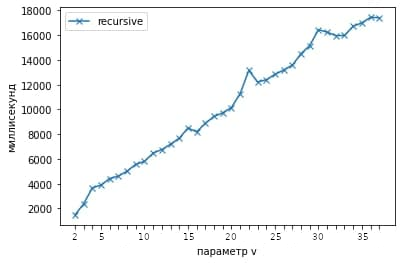
\includegraphics[width=0.8\columnwidth]{Mishin/figures/vDependenceImplicitSemiLocalSARecursie.png}
    \caption{Линейная зависимость параметра рекурсивного алгоритма semi-local SA на основе умножения липких кос }\label{fig:vParam}
\end{figure}

На Рис.~\ref{fig:speedWindow3} представлены результаты запусков двух версий алгоритмов для решения задачи Window-Substring: через предподсчет кос (\emph{implicit 350}) и наивный (\emph{naive 350})\footnote{Наивный алгоритм заключается в вычислении semi-local LCS для каждого окна $(m \times n \times w)$, где $w$~--- размер окна, $m,n$~--- размеры строк.
}.
График  показывает, что алгоритм для решения задачи Window-Substring через предподсчет кос действительно не зависит от размера окна и быстрее наивной версии.
Несмотря на это, в силу рекурсивной структуры алгоритма решения, он не применим к большим данным.

\begin{figure}[t!]
\centering
    \includegraphics[width=0.8\columnwidth]{Mishin/figures/windowNaiveImpl.png}
    \caption{Независимость от размера окна }\label{fig:speedWindow3}
\end{figure}

Таким образом, можно сделать вывод, что  при работе с большими данными может быть эффективно применён алгоритм решения задач semi-local через распутывание кос, а алгоритмы, обладающие сложной рекурсивной структурой, могут быть применены при совершении ряда оптимизаций, например, избавления от рекурсии.

%\subsection{Поиск по шаблону}
%В данной секции описаны результаты запусков различных версий алгоритмов решения \emph{задачи поиска по шаблону}. Также произведен их анализ.

%На Рис.~\ref{ssss}  представлены результаты временных замеров для  различных версий алгоритмов, решающих задачу поиска по шаблону.
%В частности, алгоритм из статьи~\cite{luciv2019interactive} (\emph{duplicate search}), его улучшенная версия, описанная в разделе~\ref{fics} (\emph{duplicate search via semi-local}), алгоритм из \emph{библиотеки алгоритмов} (\emph{ThresholdAMatch}) и алгоритм~\ref{alg:patternMathing2} с учетом замечания (см. псевдокод~\ref{alg:patternMathing2}).

%Рассматривались два сценария: меленький размер алфавита (большая частота повторов) и большой размер алфавита (маленькая частота повторов).
%В обоих случая размер текста был фиксирован и равен \emph{10000} слов.

% \begin{figure}[h]
%     \centering
%     \begin{subfigure}[b]{0.45\textwidth}
%     \centering
%     \includegraphics[width=\textwidth]{Mishin/figures/smallAlphabet.png} \caption{Сценарий с малым размером\\ алфавита}
%     \label{fig:subim1}
%     \end{subfigure}%
%     % \hfill
%     \begin{subfigure}[b]{0.45\textwidth}
%     \centering
%     \includegraphics[width=\textwidth]{figures/largeAlphabet.png}
%     \caption{Сценарий с большим размером\\ алфавита}
%     \label{fig:subim2}
%     \end{subfigure}
% \caption{Сравнение скорости различных алгоритмов решения задачи \emph{поиска по шаблону}}\label{ssss}
% \end{figure}

% График, во-первых, показывает, что алгоритм решения \emph{semi-local} может быть эффективно применен к \emph{задаче поиска по образцу}, а во-вторых, что улучшенная версия алгоритма из~\cite{luciv2019interactive} показывает лучшие результаты не только в теории, но и на практике.

\subsection{Поиск групп повторов}
В данной секции представлен анализ результатов запуска алгоритмов, решающих задачу поиска групп повторов для \textsc{JavaDoc}-документации.
Анализ производился в рамках реализованного приложения (см. главу~\ref{searchPO}).
Использовались следующие фильтры: токенизация, лемматизация, удаление стоп-слов.
Повторы искались среди \textsc{JavaDoc}-комментариев, относящихся к описанию методов, классов, интерфейсов.

Проекты, содержащие \textsc{JavaDoc}-документацию, были выбраны на основе статей, описанных в разделе~\ref{duplicateReport}.
Для нахождения групп использовался алгоритм~\ref{alg:groupDuplicate}.
В качестве функции $g$ были выбраны алгоритмы из библиотеки алгоритмов, решающие задачи bounded-length Smith-Waterman и semi-local SA.
В качестве $s$ использовались алгоритм~\ref{alg:clusterMcl} и алгоритм из~\cite{tofigh2009optimum}.
Результаты представлены в таблице~\ref{table}.

\begin{figure}[t!]

\begin{center}
 \begin{tabular}{ | p{2cm} | p{1.5cm} | p{1.5cm} | p{1.5cm} | p{1.5cm} |} 
 \hline
 \thead{Название \\ проекта} & \thead{Кол-во\\  комм.} & \thead{Кол-во\\повторов} & \thead{Кол-во\\ групп} & \thead{Время \\исп. (сек)} \\
 \hline
  \makecell{slf4j} & \makecell{188} & \makecell{157} & \makecell{25} & \makecell{8} \\
  \hline
  \makecell{apache\\ commons io} & \makecell{1284} & \makecell{1180} & \makecell{92} & \makecell{569} \\
  \hline
  \makecell{apache\\ commons\\ collection} & \makecell{610} & \makecell{495} &\makecell{50} & \makecell{408} \\
  \hline
  \makecell{gson} & \makecell{498} & \makecell{356} & \makecell{81} & \makecell{96} \\
  \hline \makecell{junit} & \makecell{680} & \makecell{539} & \makecell{87} & \makecell{163} \\
  \hline \makecell{mockito} & \makecell{2979} & \makecell{2812} & \makecell{164} & \makecell{2012}\\
  \hline \makecell{guava} & \makecell{4340} & \makecell{3662} & \makecell{418} & \makecell{8505} \\
  \hline
\end{tabular}
\end{center}
\caption{Результат работы приложения}\label{table}
\end{figure}

Пример группы одного из проектов представлен на Рис.~\ref{fig:groupViz}.
Анализ проектов с помощью приложения показал следующее.

Во-первых, построение полного графа~--- дорогостоящая операция.
Необходима предварительная фильтрация, чтобы сократить количество ребер в графе. 

Во-вторых, анализ найденных групп показал, что они преимущественно состоят из одинаковых фрагментов (одинаковые методы, схожая функциональность) с незначительными изменениями (в графе это клики).
Сложная структура дерева (без учета клик) практически не присутствует.

В-третьих, графовые алгоритмы можно применять к задаче поиска групп повторов.

В-четвертых, алгоритмы на основе решения задач semi-local также могут быть успешно применены к задаче поиска групп повторов.

Наконец, количество повторов в \textsc{JavaDoc}-документации существенно, что подтверждает результаты существующих исследований (см. раздел~\ref{duplicateReport}).

% У заключения нет номера главы
\section*{Заключение}

В данной работе исследованы существующие теоретические алгоритмы решения задач полулокального поиска наибольшей общей подпоследовательности и выравнивания строк, а также они реализованы в виде библиотеки алгоритмов на языке программирования \textsc{Kotlin}.

Также были разработаны алгоритмы решения задач поиска неточных повторов в тексте и поиска всех групп повторов.
Решения этих задач основаны прежде всего на адаптации алгоритмов из созданной библиотеки, а так же применении графовых эвристик и алгоритмов кластеризации в случае с поиском групп повторов. 

Для оценки практической применимости полученных решений было разработано приложение для поиска повторов в \textsc{JavaDoc} документации и проведена апробация на проектах с открытым исходных кодом.
Также было проведено экспериментальное исследование реализованных алгоритмов решения задачи полулокального поиска наибольшей общей подпоследовательности и выравнивания строк в контексте их применения к задачам с большим размером строк.
Результаты эксперимента показали, что часть алгоритмов имеет хорошую масштабируемость и применима к ``большим данным'', в то время как другие~--- не применимы в текущем виде, например, алгоритм муравья. 

В итоге, можно с уверенностью сказать, что полученные в ходе работы результаты являются доказательством применимости алгоритмов решения полулокальных задач к поиску повторов в документации.

\begin{thebibliography}{10}
\def\selectlanguageifdefined#1{
\expandafter\ifx\csname date#1\endcsname\relax
\else\selectlanguage{#1}\fi}
\providecommand*{\href}[2]{{\small #2}}
\providecommand*{\url}[1]{{\small #1}}
\providecommand*{\BibUrl}[1]{\url{#1}}
\providecommand{\BibAnnote}[1]{}
\providecommand*{\BibEmph}[1]{#1}
\ProvideTextCommandDefault{\cyrdash}{\iflanguage{russian}{\hbox
  to.8em{--\hss--}}{\textemdash}}
\providecommand*{\BibDash}{\ifdim\lastskip>0pt\unskip\nobreak\hskip.2em plus
  0.1em\fi
\cyrdash\hskip.2em plus 0.1em\ignorespaces}
\renewcommand{\newblock}{\ignorespaces}

\bibitem{augustsson1985compiling}
\selectlanguageifdefined{russian}
\BibEmph{Augustsson~Lennart}. Compiling pattern matching~// Functional
  Programming Languages and Computer Architecture~/ Под ред.\
  Jean-Pierre~Jouannaud. \BibDash
\newblock Berlin, Heidelberg~: Springer Berlin Heidelberg, 1985. \BibDash
\newblock {С.}~368--381.

\bibitem{myrfc}
\selectlanguageifdefined{russian}
\BibEmph{Bashkirov~Alexander}. Active patterns for OCaml. \BibDash
\newblock 2020. \BibDash
\newblock {Режим доступа}:
  \BibUrl{https://github.com/ocaml/RFCs/pull/12} ({дата
  обращения}: 01.06.2020).

\bibitem{myrepo}
\selectlanguageifdefined{russian}
\BibEmph{Bashkirov~Alexander}. Active patterns for OCaml implementation
  repository. \BibDash
\newblock 2020. \BibDash
\newblock {Режим доступа}:
  \BibUrl{https://github.com/bash-spbu/ocaml/tree/active_patterns_docker_image}
  ({дата обращения}: 01.06.2020).

\bibitem{java2019proposal}
\selectlanguageifdefined{russian}
\BibEmph{Brian~Goetz}. Data Classes and Sealed Types for Java. \BibDash
\newblock 2019. \BibDash
\newblock {Режим доступа}:
  \BibUrl{https://cr.openjdk.java.net/~briangoetz/amber/datum.html} ({дата
  обращения}: 20.05.2020).

\bibitem{emir2007objects}
\selectlanguageifdefined{russian}
\BibEmph{Emir~Burak, Odersky~Martin, Williams~John}. Matching Objects with
  Patterns~// Proceedings of the 21st European Conference on Object-Oriented
  Programming. \BibDash
\newblock ECOOP'07. \BibDash
\newblock Berlin, Heidelberg~: Springer-Verlag, 2007. \BibDash
\newblock {С.}~273--298. \BibDash
\newblock {Режим доступа}:
  \BibUrl{http://dl.acm.org/citation.cfm?id=2394758.2394779}.

\bibitem{erwig2000pattern}
\selectlanguageifdefined{russian}
\BibEmph{Erwig~Martin, Peyton~Jones~Simon}. Pattern Guards and Transformational
  Patterns~// Haskell Workshop 2000. \BibDash
\newblock 2000. \BibDash September. \BibDash
\newblock {Режим доступа}:
  \BibUrl{https://www.microsoft.com/en-us/research/publication/pattern-guards-and-transformational-patterns/}.

\bibitem{viewshaskell}
\selectlanguageifdefined{russian}
\BibEmph{GHC~Wiki}. Haskell view patterns. \BibDash
\newblock {Режим доступа}:
  \BibUrl{https://gitlab.haskell.org/ghc/ghc/wikis/view-patterns} ({дата
  обращения}: 20.05.2020).

\bibitem{unexpresiveness_example}
\selectlanguageifdefined{russian}
\BibEmph{IntelliJ~Scala}. Демонстрация
  невыразительности сопоставления на
  примере конвертера из языка Scala в UAST. \BibDash
\newblock {Режим доступа}:
  \BibUrl{https://github.com/JetBrains/intellij-scala/blob/878ef964b1bb9dc535ed0bb42ad7ea0731427065/scala/uast/src/org/jetbrains/plugins/scala/lang/psi/uast/converter/Scala2UastConverter.scala\#L366}
  ({дата обращения}: 20.05.2020).

\bibitem{kotlin2019when_expression}
\selectlanguageifdefined{russian}
\BibEmph{Kotlin~Language~Documentation}. Control Flow: When Expression.
  \BibDash
\newblock 2019. \BibDash
\newblock {Режим доступа}:
  \BibUrl{https://kotlinlang.org/docs/reference/control-flow.html\#when-expression}
  ({дата обращения}: 20.05.2020).

\bibitem{fessant2001optimizing}
\selectlanguageifdefined{russian}
\BibEmph{Le~Fessant~Fabrice, Maranget~Luc}. Optimizing Pattern Matching~//
  \href{http://dx.doi.org/10.1145/507635.507641}{\BibEmph{ACM SIGPLAN
  Notices}}. \BibDash
\newblock 2001. \BibDash 08. \BibDash
\newblock Т.~36.

\bibitem{maranget2007warnings}
\selectlanguageifdefined{russian}
\BibEmph{Maranget~Luc}. Warnings for pattern matching~//
  \href{http://dx.doi.org/10.1017/S0956796807006223}{\BibEmph{Journal of
  Functional Programming}}. \BibDash
\newblock 2007. \BibDash 05. \BibDash
\newblock Т.~17. \BibDash
\newblock {С.}~387--421.

\bibitem{maranget2008decisiontrees}
\selectlanguageifdefined{russian}
\BibEmph{Maranget~Luc}.
  \href{http://dx.doi.org/10.1145/1411304.1411311}{Compiling Pattern Matching
  to Good Decision Trees}~// Proceedings of the 2008 ACM SIGPLAN Workshop on
  ML. \BibDash
\newblock ML '08. \BibDash
\newblock New York, NY, USA~: ACM, 2008. \BibDash
\newblock {С.}~35--46. \BibDash
\newblock {Режим доступа}:
  \BibUrl{http://doi.acm.org/10.1145/1411304.1411311}.

\bibitem{csharp2019pattern_matching}
\selectlanguageifdefined{russian}
\BibEmph{Microsoft~Docs}. C\# Pattern Matching. \BibDash
\newblock 2019. \BibDash
\newblock {Режим доступа}:
  \BibUrl{https://docs.microsoft.com/en-us/dotnet/csharp/pattern-matching}
  ({дата обращения}: 20.05.2020).

\bibitem{milner1997definition}
\selectlanguageifdefined{russian}
\BibEmph{Milner~Robin, Tofte~Mads, Macqueen~David}. The Definition of Standard
  ML. \BibDash
\newblock Cambridge, MA, USA~: MIT Press, 1997. \BibDash
\newblock
  ISBN:~\href{http://isbndb.com/search-all.html?kw=0262631814}{0262631814}.

\bibitem{ocaml_iflet}
\selectlanguageifdefined{russian}
\BibEmph{OCaml~Community}. if-let for OCaml. \BibDash
\newblock {Режим доступа}:
  \BibUrl{https://github.com/ocaml/ocaml/pull/194} ({дата
  обращения}: 20.05.2020).

\bibitem{discuss}
\selectlanguageifdefined{russian}
\BibEmph{OCaml~Discuss}. Musings on extended pattern-matching syntaxes.
  \BibDash
\newblock 2019. \BibDash
\newblock {Режим доступа}:
  \BibUrl{https://discuss.ocaml.org/t/musings-on-extended-pattern-matching-syntaxes/3600}
  ({дата обращения}: 20.05.2020).

\bibitem{okasaki98views}
\selectlanguageifdefined{russian}
\BibEmph{Okasaki~Chris}. Views for Standard ML~// In SIGPLAN Workshop on ML.
  \BibDash
\newblock 1998. \BibDash
\newblock {С.}~14--23.

\bibitem{okmij_typechecker}
\selectlanguageifdefined{russian}
\BibEmph{Oleg~Kiselyov}. How OCaml type checker works -- or what polymorphism
  and garbage collection have in common. \BibDash
\newblock {Режим доступа}:
  \BibUrl{http://okmij.org/ftp/ML/generalization.html} ({дата
  обращения}: 20.05.2020).

\bibitem{pickering2016pattern}
\selectlanguageifdefined{russian}
Pattern Synonyms~/ Matthew~Pickering, Gergo~Érdi, Simon~Peyton~Jones,
  Richard~A.~Eisenberg~// Haskell'16. \BibDash
\newblock 2016. \BibDash September. \BibDash
\newblock {Режим доступа}:
  \BibUrl{https://www.microsoft.com/en-us/research/publication/pattern-synonyms/}.

\bibitem{peytonjones2020lower}
\selectlanguageifdefined{russian}
\BibEmph{Peyton~Jones~Simon, Graf~Sebastian, Scott~Ryan}. Lower your guards: a
  compositional pattern-match coverage checker. \BibDash
\newblock 2020. \BibDash March. \BibDash
\newblock In submission. {Режим доступа}:
  \BibUrl{https://www.microsoft.com/en-us/research/publication/lower-your-guards-a-compositional-pattern-match-coverage-checker/}.

\bibitem{rust_reference}
\selectlanguageifdefined{russian}
{The Rust reference}~: Intern report~/ {Inria}~; {исполн.}:
  Community~Rust~: 2020. \BibDash
\newblock {Режим доступа}:
  \BibUrl{https://doc.rust-lang.org/reference/index.html}.

\bibitem{scott2000whendo}
\selectlanguageifdefined{russian}
\BibEmph{Scott~Kevin~D, Ramsey~Norman}. When Do Match-compilation Heuristics
  Matter?~// Technical Report CS-2000-13. \BibDash
\newblock 2000.

\bibitem{syme2007extensible}
\selectlanguageifdefined{russian}
\BibEmph{Syme~Don, Neverov~Gregory, Margetson~James}. Extensible pattern
  matching via a lightweight language extension~// Proceedings of the 12th ACM
  SIGPLAN international conference on Functional programming. \BibDash
\newblock Association for Computing Machinery, Inc., 2007. \BibDash October.
  \BibDash
\newblock {Режим доступа}:
  \BibUrl{https://www.microsoft.com/en-us/research/publication/extensible-pattern-matching-via-a-lightweight-language-extension/}.

\bibitem{leroy2019manual}
\selectlanguageifdefined{russian}
{The OCaml system release 4.09: Documentation and user's manual}~: Intern
  report~/ {Inria}~; {исполн.}: Xavier~Leroy, Damien~Doligez,
  Alain~Frisch и~др.~: 2019. \BibDash Сент. \BibDash
\newblock {С.}~1--789. {Режим доступа}:
  \BibUrl{https://hal.inria.fr/hal-00930213}.

\bibitem{tullsen2000firstclass}
\selectlanguageifdefined{russian}
\BibEmph{Tullsen~Mark}. First Class Patterns~// In 2nd International Workshop
  on Practial Aspects of Declarative Languages, volume 1753 of LNCS. \BibDash
\newblock Springer-Verlag, 2000. \BibDash
\newblock {С.}~1--15.

\bibitem{wadler1987views}
\selectlanguageifdefined{russian}
\BibEmph{Wadler~P.} \href{http://dx.doi.org/10.1145/41625.41653}{Views: A Way
  for Pattern Matching to Cohabit with Data Abstraction}~// Proceedings of the
  14th ACM SIGACT-SIGPLAN Symposium on Principles of Programming Languages.
  \BibDash
\newblock POPL '87. \BibDash
\newblock New York, NY, USA~: ACM, 1987. \BibDash
\newblock {С.}~307--313. \BibDash
\newblock {Режим доступа}:
  \BibUrl{http://doi.acm.org/10.1145/41625.41653}.

\end{thebibliography}




